\documentclass[letterpaper,12pt]{article}

\usepackage[tocbib,bibnewpage]{apacite}
\usepackage{graphicx}
\usepackage{rotating}
\usepackage{color}
\definecolor{lightgrey}{rgb}{.5,.5,.5}
\usepackage{tabularx}
\usepackage{appendix}
\usepackage{longtable}
\usepackage{url}

\usepackage{myapa}
\FiveLevelHeading
\raggedright
\setlength{\parindent}{0.3in}

\newcommand{\smaller}{\fontsize{9}{10}\selectfont}

\usepackage{setspace}
\doublespacing


\def\quote{\singlespacing\parindent2em\hangindent2em}

\oddsidemargin 0.0in
\evensidemargin 0.0in
\textwidth 6.5in
\headheight 0.0in
\topmargin 0.0in
\textheight 8.5in
\doublerulesep 0pt
\newcommand{\thickline}{\hline\hline\hline}

%\pagenumbering{roman}
\renewcommand*\contentsname{Table of Contents}

\begin{document}
\begin{titlepage}
\vspace*{\fill}
\begin{center}
\uppercase{A National Study Comparing Charter and Traditional Public Schools Using Propensity Score Analysis}\\
\ \\
by
\ \\ \ \\
Jason M. Bryer\\
\ \\ \ \\ \ \\
A Dissertation Proposal\\
Submitted to the University at Albany, State University of New York\\
In Partial Fulfillment of\\
the Requirements for the Degree of\\
Doctor of Philosophy\\
\ \\ \ \\ \ \\ \ \\
School of Education\\
Department of Educational and Counseling Psychology\\
Division of Educational Psychology \& Methodology\\
2012
\end{center}
\vspace*{\fill}
\end{titlepage}
\setcounter{page}{2}
\newpage

\section{Abstract}

The concept of school choice within the United States is not new. Private schools have been educating students since the founding of the United States. However, in 1988, Ray Budde proposed an alternative approach to school choice that has come to be known as charter schools \cite{Kolderie2005}. Unlike their private school counterparts, charter schools receive public funding, but they are relieved of many of the bureaucratic and regulatory constraints public schools adhere to, but are still held accountable for student performance. Despite claims by charter school advocates that charter schools are performing as well if not better than the public school counterparts \cite<see e.g.>{AllenConsolettieKerwin2009}, studies provide mixed results with regard to charter school performance \cite<see e.g.>{BraunJenkinsGrigg2006, credo, HubbardKulkarni2009}. Ultimately, there is agreement that more research is necessary to address the question of how charter schools perform with respect to their academic outcomes for students. 

This dissertation has two major goals: 1. To develop new methods, largely graphical in form, to facilitate multilevel or cluster analyses of observational data while accounting for covariate differences between the groups being compared, and 2. to use these new methods using a large archival data base to compare outcomes for students who attend charter schools with their traditional public school counterparts on two key academic domains: reading and mathematics. 

The new methods represent extensions of modern methods for propensity score analysis (see below) that aim to reduce if not eliminate selection bias in the context of clustered data. Charter schools are, by definition, schools of choice; traditional public schools are, at least by default, also schools of choice. This means that observational data methods are needed to compare these two kinds of schools with one another because students (or their parents) who choose between these two kinds of schools tend to be systematically different from one another with respect to multiple covariates. That is, comparisons of these two kinds of schools tend to be afflicted by selection bias, or as in this case, the likely systematic differences introduced due to the lack of randomization of students being placed in either of the two groups.. Given well designed observational studies, and appropriate analysis methods, effects of the selection bias may be reduced, if not eliminated. The advent of new methods for observational data analysis will generally result in ways to replace simple comparisons of two independent groups by comparisons that make adjustments for covariate differences. In the present context the new methods do this chiefly using graphical methodologies.

New statistical procedures for observational data analysis introduced by \citeA{RosenbaumRubin1983} called propensity score analysis. Propensity score analysis has seen considerable increased use in the social sciences within the last few years \cite{ArpinoMealli2008}. However, its development and use in situations where multilevel, or clustered data are of interest, have been limited \cite{ThoemmesKim2011}. 									

Using data from the 2007 and 2009 National Assessment of Educational Progress (NAEP) for mathematics and reading at grades four and eight, estimates of the differences between charter and public schools will be calculated at two levels, namely state and national. Given the variability of charter schools laws across states, it is important to consider the impact of clustering. Analyses will be conducted using the newly developed \texttt{multilevelPSA} package \cite{multilevelPSA} in R \cite{rdevelopment}. Specifically, propensity scores will be estimated within each state and these will be used for matching or stratification of students within each state. Comparisons of specific students, or groups of students, will in all cases be done within states. Effects will then aggregated to provide state and national effect estimates.

As with all propensity score analyses, it is preferable to utilize multiple methods for estimating propensity scores \cite<see e.g.>{Stuart2010}. Doing so can help to provide confidence that results reflect what the data have to say, and is not merely an artifact of model specification or method choice. This study will utilize three overall approaches to propensity score analysis, namely stratification, matching, and multilevel stratification. Lastly, the use of graphics will be employed to evaluate balance and outcome differences using methods (functions) found in \citeA{HelmreichPruzek2009}.

\newpage 

\section{Introduction}

Since the opening of the first charter school in Minnesota in 1991, the United States\footnote{Though this study focuses on charter schools in the U.S., Canada \cite{canada2007}, Chile \cite{Larranaga2004}, England \cite{WohlstetterAnderson1994}, Germany \cite{Herbst2006}, and New Zealand \cite{Lander2001} also have charter schools.} has increasingly embraced charter schools as an option for educational reform. In the last 10 years for which data are available, the number of charter schools grew from 507 in the 1998-1999 school year to 4,561 in the 2007-2008 school year \cite<see figure \ref{fig:charterSchoolGrowth};>{cernumbers}. Currently, 40 states and the District of Columbia have charter school laws (see appendix A for enrollment by state \& Appendix B for a thematic map of the U.S. depicting the number of operating charter schools as of 2008). And, given charter school supporter Arne Duncan's appointment as Secretary of Education by President Barack Obama, charter school growth seems likely to continue in the near future.

In principle, charter schools opt out of bureaucratic rules and union contracts in order to gain administrative autonomy. The standard argument has become that this autonomy will lead to higher student test scores and better academic environments \cite{Wells2002} because in the charter framework, teachers, administrators, students and the community that comprise charter schools are free to innovate. Proponents argue that charter schools are more likely than their conventional counterparts to serve as experimental schools where the innovations can inform reform of public education at large. Some charter supporters even envision a time when most traditional public schools will be replaced by charter schools. This is exemplified by the attempted school voucher legislation during the second G.W. Bush Administration.

\begin{figure}[tp]
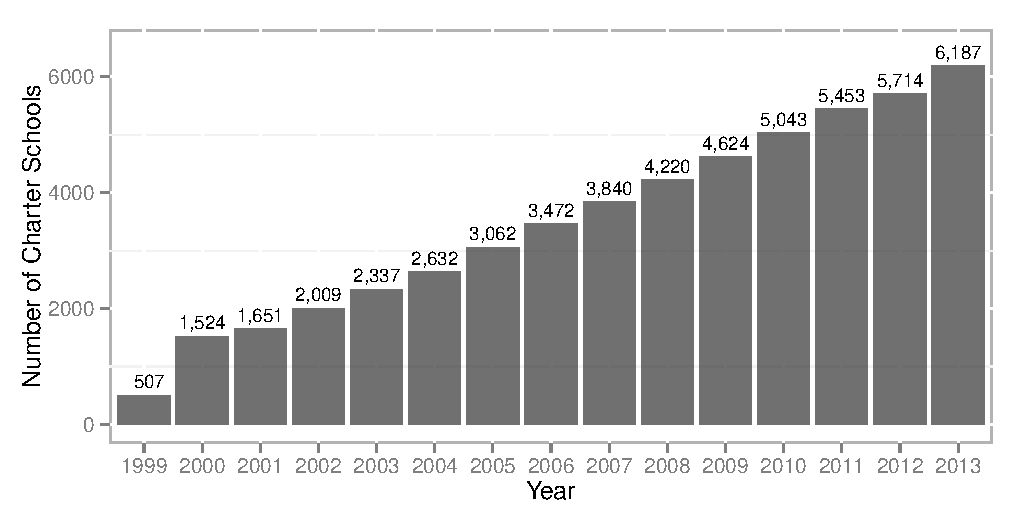
\includegraphics[width=\textwidth]{../Figures/CharterSchoolGrowth.pdf}
\caption{Charter School Growth 1999-2008}
\label{fig:charterSchoolGrowth}
\end{figure}

Clearly charter schools have become a popular vehicle among parents. The \citeA{cersurvey} reports that 59\% of charter schools have waiting lists averaging 198 students.   Charter schools seem to have provided an apparent choice to many parents and are congruent with the United State�s individualistic \cite<see e.g.,>{Hofstede2004,Maccall1847,Swart1962} culture.

%Proponents of charter schools argue that traditional public schools have been bogged down by bureaucracy and union contracts. Freeing schools of these requirements then allows teachers and schools to innovate, which in theory leads to increased student performance. The principled argument is the ``market metaphor" \cite{Wells2002}. That is, if schools were forced to compete for ``customers" (i.e. students), then the differentiating factor between schools would be the quality of education. 

Whatever the generic arguments supporting charter schools in the U.S., it is clear that sound empirical evidence is needed to evaluate this class of schools in relation to their traditional counterparts. Several studies have shown that charter schools are not only failing to increase student performance, but in fact often perform well below their traditional public school counterparts in terms of achievement test scores \cite<see e.g.,>{credo,BraunJenkinsGrigg2006,aft2004}. Others still argue whether charter schools may be a solution in search of a problem. \citeA{Carnoy2005} in summarizing the controversy that ensued after the \citeA{aft2004} study argue that:

\begin{quote}    %Good quote... come back to the idea at some point!
If, however, charter schools are not improving the achievement of disadvantaged children, it may be that the cause of low student performance is not bureaucratic rules but something else. When a treatment is based on a diagnosis, and the treatment doesn't work, it is prudent to examine not only whether the treatment should be improved, but also whether the diagnosis might be flawed. \cite{Carnoy2005}
\end{quote}

\subsection{Issues with Charter School Research}
A large number of issues surround the topic charter schools, including their nature or form, their settings and especially their curricula. Given the numbers of current and future generations of students for which decisions about charter schools have central implications, one key concern must certainly be that of comparative outcomes of charter in relation to traditional public schools. Clearly, this issue should be explored using the best and most comprehensive data and methods available. \citeA{BettsHill2006} identify three major obstacles to addressing the question of �whether students in charter schools are learning more or less than they would have learned in conventional schools" (p. 1), namely:

\begin{enumerate}
\item The issue of selection bias\footnote{\citeA{BettsHill2006} cite counterfactuals as the issue. Though the issue of counterfactals is an important concept in defining causal inference, it is problematic from a practical viewpoint. Specifically, it is impossible to observe two treatment conditions (or treatment and non-treatment) on the same individual \cite<i.e. ``the fundamental problem of causal inference",>{Holland1986}.}.

\item The variation in types or kinds of charter schools (and the rules under which they operate in different states).

\item The nature of student achievement. Research has shown there are numerous factors that contribute to student success including, but not limited to, social economic status, parental education, motivation, etc. The ability to decipher how school choice contributes to student learning in the context of all the other factors cannot help but be difficult. 
\end{enumerate}

\noindent All of these issues are significant, but some are only partially amenable to empirical study, and some must be addressed in future research. We shall in fact focus on only a subset of these issues, and will do so only with respect to one large archival data set. Given the need for evidence regarding the relative performance of charter schools in relation to their conventional public school counterparts, we will focus on how effectively to use a large archival data set to ameliorate the effects of selection bias in the comparison of these two kinds of schools. The limitations of such study should also become clear, and will be discussed in some detail.

As noted above, selection bias will be examined in some detail. However, the central point is easy to state: statistical methods that incorporate propensity scores can provide ways to adjust for manifest selection bias in observational studies. It follows that under certain conditions, treatment comparisons, such as the comparison of charter and conventional public schools, can be clarified by reducing confounding effects through the use of covariates. In idealized conditions, interpretations of observational group comparisons can approach the qualities of randomized experiments with respect to the key goal of supporting causal inferences. To the extent that idealized conditions fail to exist or be reached, results of observational study comparisons will tend to become unclear, which is to say that confounding effects may continue to play a notable role. (While observational study comparisons may fail to provide sound causal evidence the same can be said for for true experiments, that is for studies where random assignments to groups have been employed. Of course the fundamental problem of causal inference remains \cite{Holland1986}. That is, it is impossible to observe treatment and non-treatment on the same unit of analysis.

The second issue noted above, that the term �charter school" means different things in different contexts, is often cited in critiques of national or large-scale charter school studies. The same of course is also true of public schools!  However, to suggest that such variations obviate meaningful comparisons of these two fundamentally different kinds of schools would be an extreme judgment, one that when generalized would preclude or at least hinder all school (type) comparisons. It is a key assumption of the proposed dissertation that meaningful comparisons of charter and public schools does not require that each type be in any sense �pure.�

Given that the charter school debate is national, and has implications at the Federal level, large scale studies are not only likely to be useful, they are necessary because charter schools are routinely being offered, with few exceptions, as alternatives to traditional public schools, throughout the nation. For the few states that don�t currently have charter schools, incentives at the federal level for states to have charter schools have been put forth (e.g. the Race to the Top Initiative). In the case of this work the aim is not to focus on particular charter schools, or types of charter schools, but rather to compare these kinds of schools under one broad umbrella using government sponsored archival data that derives from carefully developed tests. The specific focus is on outcomes for the subjects reading and mathematics, using data aggregated at the level of the states.

Lastly, the roles of environmental, social, community, and cultural factors that contribute to a student�s academic achievement are often ignored or underestimated. Often educational reform, as exemplified most recently by the No Child Left Behind Act, places the responsibility solely on the school without consideration of the context in which the school operates. 

Although educators acknowledge that schools, in their various forms, are only part of what contributes to student academic achievement, they are nevertheless important parts and it behooves educators to evaluate school effects quite generally. The particular approach used there is to compare school effects using a class of statistical methods that should make it possible to make clearer, less qualified conclusions, than is usually has been possible. 

\subsection{Research Questions \& Objectives} 
The primary focus of this study is the development of a new set of methods for propensity score analysis with multilevel, or clustered, data. One of these aims is to show how graphics can be used to address research questions in the context of multilevel propensity score analysis; another is to describe and illustrate the key features of a new package of R functions to facilitate multilevel propensity score analyses, vis-\`{a}-vis the \texttt{multilevelPSA} package in R. Moreover, these new multilevel methods for propensity score analysis will be presented within the context of more traditional methods for propensity score analysis, namely stratification and matching. Not only will this show how these new methods perform with regard to more established methods, they may show with the use of modern graphics, how clusters may vary. 

The newly developed multilevelPSA package will be shown to provide an effective means of estimating and visualizing propensity score results with clustered (multilevel) data (these procedures are discussed more fully below; see also Figure 2). Moreover, the use of pre-existing visualization procedures such as loess regression plots, density plots, as well as the PSA balance and assessment plots introduced by \citeA{HelmreichPruzek2009}, can provide critical insight into the analysis and eventual interpretation of results. More succinctly, the presentation of graphics in this study are not merely provided for diagnostic or descriptive purposes, but are a critical component of presenting, analyzing, and interpreting results. For instance, related to research questions two and three below, it is the graphics that will be most revealing in the differences, if any, and not the numerical analyses (though numerical analyses are provided).

Given that charter schools are regularly being offered as solutions for needed educational reform nationally, it is imperative that they be evaluated from a national perspective. This study proposes to compare the academic performance in two domains of charter and traditional public schools using the National Assessment of Educational Progress (NAEP) using multiple propensity score methods. More specifically, this study proposes to address the questions:

\begin{enumerate} 
	\item Given appropriate adjustments based on available student data, is there a discernible difference between charter and traditional public schools with regard to math and reading scores at grades 4 and 8?
	\item If so, what is the nature and magnitude of this difference for the two outcomes reading and mathematics (for two grade levels)?
	\item And finally, how, and how much do identified differences differ between states with differing charter school laws?
\end{enumerate}

\section{Method}
In this section I outline methods that will be utilized to describe and analyze the data in order to address the research questions central to this study. Given the strong political interests in the question of charter school effectiveness and the implications for educational policy both at the state and national level, obtaining sound and interpretable empirical evidence, preferably with support for causal inferences, is most desirable. 

The \textit{gold standard} of applied scientific research is the randomized experiment. A research design that addresses the charter school question proposed here would require that students be randomly assigned, possibly with blocking on key covariates, to either a charter or traditional public school. The theoretical justification for such a scheme is that any systematic differences between the two groups would be balanced through the randomization process. However, in practice, randomization is rarely feasible, and may not be ethical in the context of comparing charter and traditional public schools. This introduces a phenomenon called selection bias, which refers to systematic covariate differences between the groups being compared, differences that tend to confound interpretations of comparative results. That is, any comparison of the two groups is likely to be biased given the fact that the units of study, are likely to be systematically different from one another on one or more covariates; such differences, in turn, generally make it impossible to interpret effects due to this confounding. 

Propensity score analysis \cite{RosenbaumRubin1983} is a statistical methodology whereby the covariate differences between the two groups are, in large measure, taken into account. This is done through use of a method that uses available covariate information to construct propensity scores for each unit (student); comparisons are then made between the groups, conditional on the derived propensity scores. 

In the case of this study the general approach being used is based on archival data, so it is retrospective, not prospective approach (where covariates are defined and measured by the investigator at the outset). In retrospective studies the investigator is limited to covariate data that was collected and included in the archive. Fortunately, in the case of the NAEP archive, extensive covariate information is available, which strengthens the case for using propensity score methods. Furthermore, the general procedure lends itself well to secondary analysis of the available observational data.

\subsection{Overview of NAEP}
The source of the data that will be utilized in this study is provided by the National Center for Educational Statistics (NCES) which is within the U.S. Department of Education�s Institute of Education Sciences (IES). The National Assessment of Educational Progress (NAEP) was started in 1971 and has regularly provided national measures of student achievement in many subjects including mathematics, reading, science, writing, history, civics, and the arts since its inception. In 2003 NAEP began assessing charter schools as well as private and public schools. This study will utilize the 2007 and 2009 administration of the NAEP assessments in mathematics and reading within grades four and eight. The 2007 assessment included over 6,000 public schools and over 200 charter schools comprising of over 145,000 and 3,000 students, respectively. Given this relatively large, nationally representative sample, analysis of NAEP assessments utilizing propensity score analysis may provide valuable insights into the academic differences between charter and traditional public schools.

More than simply providing large samples, another key advantage of NAEP is the fact that it is not designed to assess individual students or schools, but instead to inform broadly about subject-matter achievement, instructional experiences, and school environments for states and regions in the U.S. (Braun, Jenkins, \& Grigg, 2006). To achieve this goal, NAEP utilizes a complex item-sampling design such that individual students are presented a subset of the total items, thereby reducing the burden on individual participants. Though not appropriate for assessing individual student achievement, in aggregate the NAEP measures provide statistically and psychometrically sound estimates of large group similarities and differences in student achievement.

In addition to subject area measures, NAEP includes student, teacher, and school questionnaires that provide contextual information about the students� environment. In addition to typical demographic items such as gender and race, students are asked about computers, books, magazines, and encyclopedias in the home; parents education level; and the level of interaction with academics within the home (see Appendix C for complete list of items).

The answers to items on these questionnaires provide the covariate information that will be used in PSA to adjust for selection bias. Propensity scores will be derived from the covariates to construct student propensity scores (e(x)), these being estimates of the probability of being in the treatment group (i.e. charter school in the context of this study). The complement of each propensity score, 1 - e(x), estimates the probability of being in a traditional public school, based on available covariates. The responsibility for developing the assessment objectives and test specifications lies with the National Assessment Governing Board that was created by Congress in 1988. The governing board is charged with deciding what are appropriate achievement goals, nationally, and state-by-state, for each age and grade. The following two sections provide the framework for mathematics and reading assessments.

\subsection{Analysis}
Most of the studies conducted using PSA involve analysis in two phases where phase one involves the calculation of propensity scores or matching for both treatment and control units of analysis; and phase two involves the comparison of those two groups. However, there is little research with regard to situations where data is multilevel. As such, this study will be organized as follows:

\begin{enumerate}
	\item \textit{Propensity score analysis using stratification.} This method ignores state assignment as a clustering variable. Under this broader method three statistical methods for stratification will be used:
		\begin{enumerate}
			\item Full logistic regression. This method will estimate propensity scores using logistic regression with all available covariates.
			\item Logistic regression with step AIC. The \texttt{stepAIC} in the \texttt{MASS} package \cite{mass} will select the best logistic model based upon the Akaike Information Criterion \cite{Akaike1974}. In this case the �best� first order interaction terms will be added to the main effect terms in a.
			\item Conditional inference trees, based on all covariates; missing data will also be accommodated with the tree-based methods.\footnote{Random forest methods based on trees would, according to the available literature be more desirable that simple trees, but the large number of `clusters' (states) and the relatively large sample size here make this option too time-consuming to consider.}
		\end{enumerate}
	\item \textit{Propensity score matching.} This method implicitly accounts for clustering. That is, the method used will find matches between treated and control units that first match exactly on state, ethnicity, and gender, then finds a best match based upon the propensity scores estimated using logistic regression. As suggested by \citeA{Stuart2010}, multiple matched sets will be formed using (charter-to-traditional public school students):
		\begin{enumerate}
			\item One-to-one
			\item One-to-five
			\item One-to-ten.
		\end{enumerate}
		A dependent sample analysis will be performed on the resulting matched pairs \cite{Austin2011}.
	\item \textit{Multilevel propensity score analysis.} This method will utilize the same stratification methods as described in method one above, namely:
		\begin{enumerate}
			\item Full logistic regression.
			\item Logistic regression with step AIC.
			\item Conditional inference trees.
		\end{enumerate}
	However, where this method differs from method one is that separate models will be estimated for each state separately. Results from each state are then aggregated to provide an overall, national estimate of the differences between charter and traditional public school. Moreover, this method provides an approach whereby differences between meaningful subgroups (states in this study) can be explored, especially with the use of graphics as described below.
\end{enumerate}

It is generally recommended that multiple methods for the estimation of propensity scores be used \cite<see e.g.>{StuartRubin2008,Stuart2010}. The choices of methods for this study were chosen first to provide estimations disregarding clustering, to utilize clustering implicitly, and to utilize clustering explicitly. Then secondly, within each of these three approaches with respect to clustering, multiple methods are used in accordance to the recommendations provided by \citeA{StuartRubin2008} and \citeA{Stuart2010}. 

\begin{figure}[tp]
\begin{center}
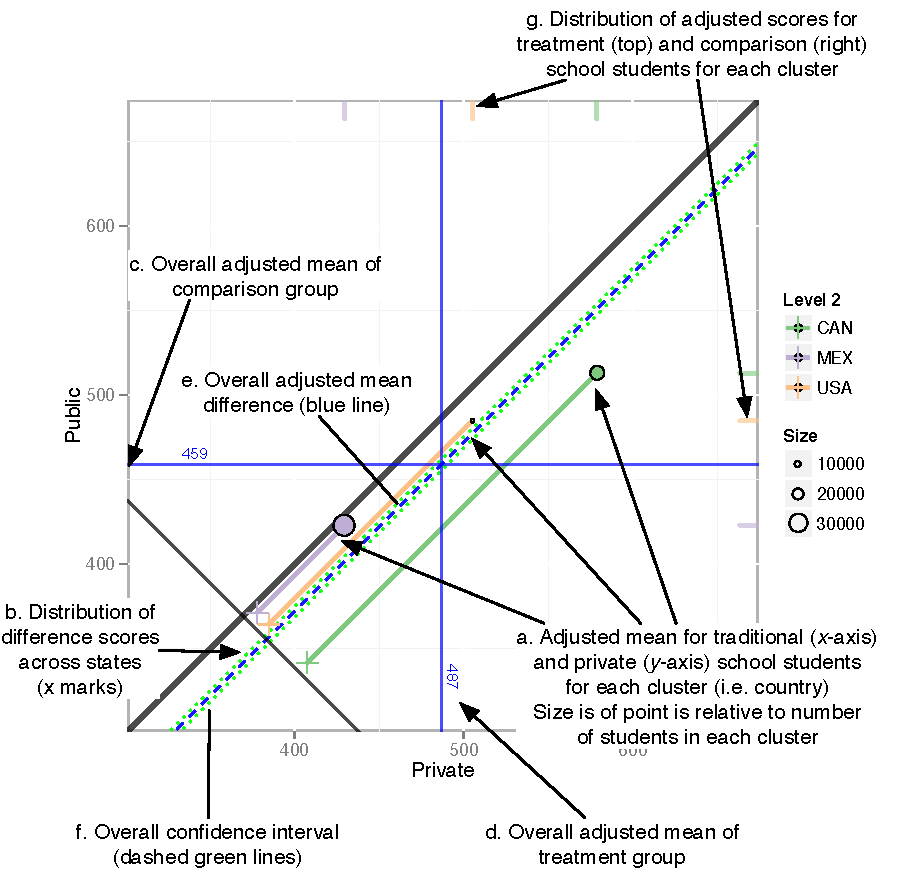
\includegraphics[width=\textwidth]{../Figures/AnnotatedCircPlot.pdf}
\caption{Multilevel PSA Assessment Plot}
\label{fig:g8math:circ}
\end{center}
\end{figure}

\subsection{Visualizing Multilevel PSA}

Given the large amount of data that needs to be summarized, the use of graphics will be an integral component of representing the results. The \texttt{multilevelPSA}\footnote{The \texttt{multilevelPSA} package was written by the author and is available from \url{http://github.com/jbryer/multilevelPSA}.} package provides a number of graphing functions that extend the framework introduced by \citeA{HelmreichPruzek2009} for multilevel PSA. Figure \ref{fig:g8math:circ} represents a multilevel PSA assessment plot with annotations. In this graphic, the x-axis corresponds to traditional public school grade 8 NAEP scores and the y-axis corresponds to charter school grade 8 NAEP scores. Each colored circle (a) is a state with its size corresponding the number of students within each state. Each state is projected to the lower left, parallel to the unit line, such that a tick mark is placed on the line with slope -1 (b). These tick marks represent the distribution of differences between charter and traditional public schools across states. Differences are aggregated (and weighted by size) across states. For grade 8 math, the overall adjusted mean for charter school students is 278 and the overall adjusted mean for traditional public school student is 278 and represented by the horizontal (c) and vertical (d) blue lines, respectively. The dashed blue line parallel to the unit line (e) corresponds to the overall adjusted mean difference and likewise, the dashed green lines (f) correspond to the confidence interval. Lastly, rug plots along the right and top edges of the graphic (g) correspond to the distribution of each state's overall mean charter and traditional public school NAEP scores, respectively.

Figure \ref{fig:g8math:circ} represents a large amount of data and allows provides much greater insight into the data and results. The figure provides overall results that would be present in a traditional table, for instance the fact that the green dashed lines span the unit line (i.e. y = x) indicates that there is a non-significant difference between the two groups. However additional information is difficult to convey in tabular format. For exmaple, the rug plots indicate that the variance in the performance of charter schools is much greater than that of traditional public schools. We can also observe that most states cluster near the overall mean (i.e. where the vertical and horizontal blue lines intersect), but there are a few states that perform well below the rest of the states (namely those located towards the bottom left of the figure). These are of particular interest due to the fact that theese states are among those with the greatest difference in favor of charter schools. That is, the states where charter schools are performing substantially better than their traditional public school counterparts are overall performing substaintly worse than other states.

\begin{figure}[t]
\begin{center}
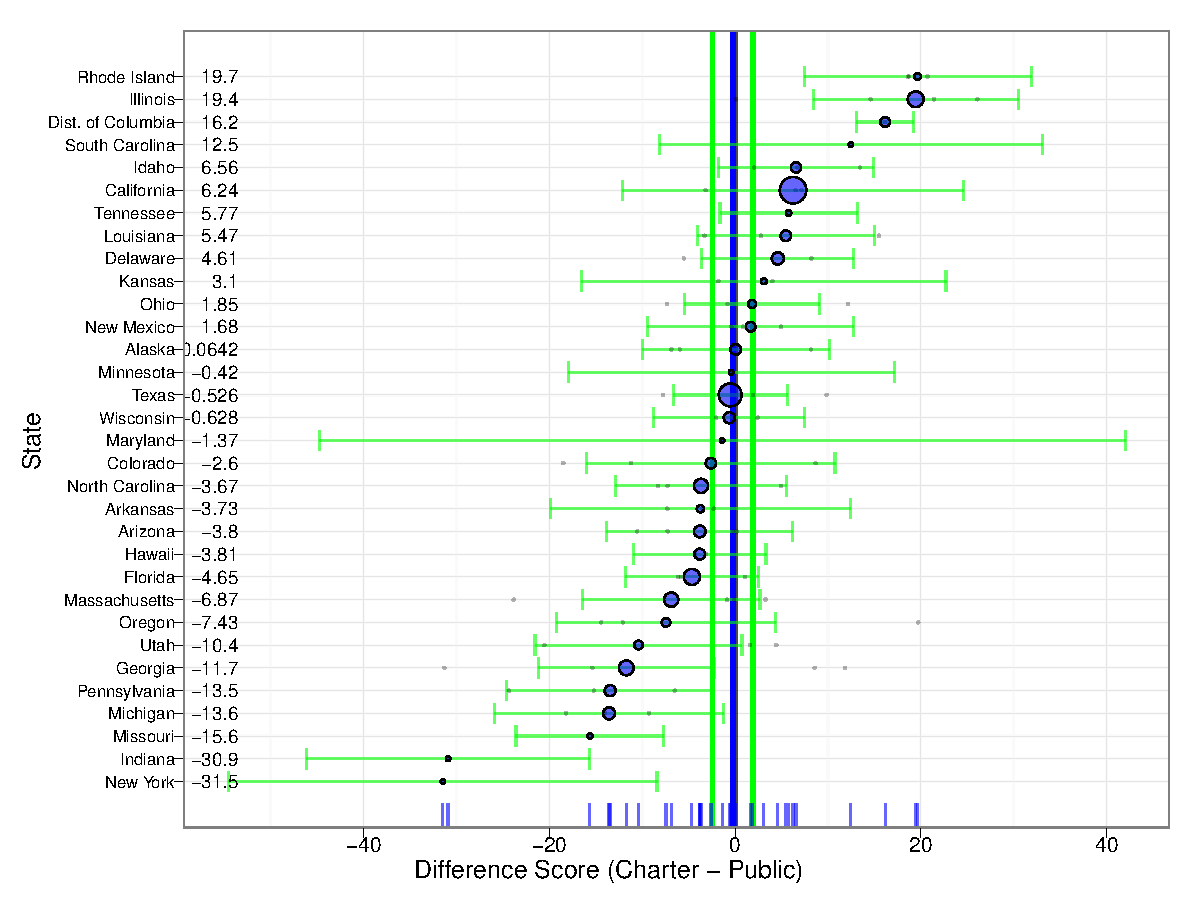
\includegraphics[height=4in]{../Figures/g8mathlrdiffplot.pdf}
\caption{Multilevel PSA Difference Plot: Grade 8 Math}
\label{fig:g8math:diff}
\end{center}
\end{figure}

Figure \ref{fig:g8math:diff} provides a more nuanced depiction of the differences both between and across states. Similar to the mutlielvel PSA assessment plot, each blue dot corresponds to a state and is sized relative to the number of students within each state. The light gray dots correspond to each strata within each state. The graphic also provides confidence intervals for each state as well as the overall adjusted mean difference (the vertical blue line) and confidence interval (the vertical green lines).

\section{(Preliminary) Results}

The tables and figures in this section represent the preliminary results of the analysis outlined in the methods section. Though these results will likely differ than the results reported in the final dissertation, they provide sufficient approximations. 

Figure \ref{fig:overallresults} provides a summary of all the results across the four dependent variables. This graphic displays the mean adjusted differences as blue dots with the confidence interval in green. Therefore, any instance where the confidence interval does not cross zero (as represented by the vertical black line) indicates there is a statistical significant difference. Tables 10, 11, and 12 in Appendix K provide the overall numerical results, that provide the basis for Figure \ref{fig:overallresults}, for each dependent variable (i.e. math and reading at grades 4 and 8) using stratification, matching, and multilevel PSA, respectively. 

Examining Figure \ref{fig:overallresults}, I see there is general agreement across the nine different methods used. That is, given the various approaches to adjusting selection bias with the available student information provides consistent conclusions. Specifically, these results suggest there is no statistical difference between charter and traditional public school students in grade 4 math and reading. Grade 8 math provides mixed results whereby five of the nine methods have confidence intervals that do not span zero. For grade 8 reading however, there is a clear statistical difference as all nine methods result in confidence intervals that do not span zero (effect size $\le$ .20).

\begin{figure}[t]
\begin{center}
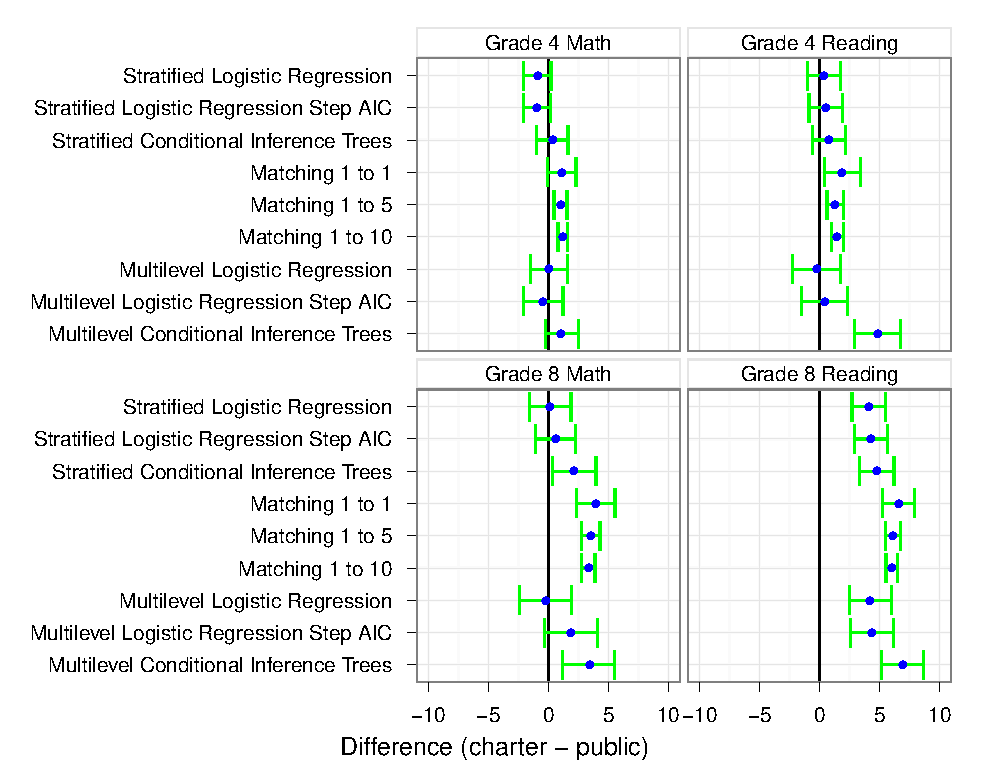
\includegraphics[height=4in]{../Figures/overallsummary.pdf}
\caption{Summary of Overall Results}
\label{fig:overallresults}
\end{center}
\end{figure}



%==================== REFERENCES ====================================================================
\cleardoublepage
\bibliographystyle{apacite}
\bibliography{Bibliography}

\newpage

%==================== Appendices ====================================================================
\cleardoublepage
\addcontentsline{toc}{section}{Appendices}
\appendix

%==================== Appendix A ====================================================================
\renewcommand{\thefootnote}{\fnsymbol{footnote}}% Change the footnote style to lowercase letters
\addcontentsline{toc}{subsection}{Appendix A: Charter School \& Student Enrollment by State}
\subsection*{Appendix A\\Charter Schools \& Student Enrollment by State}
\label{appendixCharterStats}
\begin{center} \begin{singlespace}
\begin{longtable}{lrrrrrrr}
\caption[Charter Schools \& Student Enrollment by State]{Charter Schools \& Student Enrollment by State} \\
\thickline
      & Law     & \multicolumn{3}{c}{Totals for Charter Schools\tabfnm{b}}              & & \multicolumn{2}{c}{NAEP Students}\\
\cline{3-5} \cline{7-8}
State & Enacted & Operating & Closed & Students & & Charters & Publics\\
\hline
\endfirsthead
\multicolumn{8}{l}{Charter Schools \& Student Enrollment by State (cont.)}\\
\hline
      & Law     & \multicolumn{3}{c}{Totals for Charter Schools\tabfnm{b}}              & & \multicolumn{2}{c}{NAEP Students}\\
\cline{3-5} \cline{7-8}
State & Enacted & Operating & Closed & Students & & Charters & Publics\\
\hline
\endhead
\hline 
\endfoot
\thickline
\endlastfoot
Alabama\tabfnm{a}       &      & 0   & 0   & 0       & &   0 & 2759\\
Alaska                  & 1995 & 26  & 5   & 5,198   & &  69 & 2517\\
Arizona                 & 1994 & 510 & 96  & 119,903 & &  99 & 2674\\
Arkansas                & 1995 & 25  & 6   & 6,750   & &  30 & 2407\\
California              & 1992 & 802 & 103 & 316,468 & & 417 & 7803\\
Colorado                & 1993 & 151 & 10  & 54,497  & & 108 & 2598\\
Connecticut             & 1996 & 21  & 5   & 3,932   & &   0 & 2531\\
Delaware                & 1995 & 21  & 2   & 8,740   & & 180 & 2641\\
Washington DC           & 1996 & 93  & 16  & 25,385  & & 652 & 1336\\
Florida                 & 1996 & 382 & 82  & 108,382 & & 175 & 3876\\
Georgia                 & 1993 & 83  & 5   & 40,807  & &  64 & 3465\\
Hawaii                  & 1994 & 32  & 0   & 7,317   & & 132 & 2605\\
Idaho                   & 1998 & 32  & 1   & 10,492  & &  59 & 2784\\
Illinois                & 1996 & 74  & 8   & 27,683  & &  33 & 4015\\
Indiana                 & 2001 & 50  & 2   & 12,631  & &  11 & 2720\\
Iowa                    & 2002 & 10  & 0   & 1,462   & &   0 & 2839\\
Kansas                  & 1994 & 40  & 10  & 3,361   & &  17 & 2726\\
Kentucky\tabfnm{a}      &      & 0   & 0   & 0       & &   0 & 2696\\
Louisiana               & 1995 & 66  & 10  & 23,634  & &  97 & 2264\\
Maine\tabfnm{a}         &      & 0   & 0   & 0       & &   0 & 2658\\
Maryland                & 2003 & 34  & 2   & 7,301   & &   6 & 2825\\
Massachusetts           & 1993 & 64  & 6   & 23,905  & &  56 & 3667\\
Michigan                & 1993 & 250 & 27  & 94,092  & & 134 & 2480\\
Minnesota               & 1991 & 159 & 29  & 28,371  & &  16 & 2875\\
Mississippi             & 1997 & 1   & 0   & 367     & &   0 & 2613\\
Missouri                & 1998 & 39  & 5   & 13,125  & &  38 & 2771\\
Montana\tabfnm{a}       &      & 0   & 0   & 0       & &   0 & 2581\\
Nebraska\tabfnm{a}      &      & 0   & 0   & 0       & &   0 & 2688\\
Nevada                  & 1997 & 26  & 7   & 7,295   & &   0 & 2662\\
New Hampshire           & 1995 & 11  & 2   & 1,212   & &   0 & 2803\\
New Jersey              & 1996 & 64  & 19  & 17,986  & &   0 & 2813\\
New Mexico              & 1993 & 70  & 3   & 11,426  & &  54 & 2722\\
New York                & 1998 & 118 & 10  & 32,602  & &  16 & 3745\\
North Carolina          & 1996 & 103 & 32  & 30,445  & &  72 & 4090\\
North Dakota\tabfnm{a}  &      & 0   & 0   & 0       & &   0 & 2307\\
Ohio                    & 1997 & 293 & 48  & 94,171  & &  45 & 3746\\
Oklahoma                & 1999 & 14  & 1   & 4,770   & &   0 & 2612\\
Oregon                  & 1999 & 93  & 8   & 13,612  & &  41 & 2626\\
Pennsylvania            & 1997 & 133 & 12  & 61,823  & &  64 & 2709\\
Rhode Island            & 1995 & 11  & 0   & 2,894   & &  30 & 2621\\
South Carolina          & 1996 & 36  & 10  & 8,705   & &  16 & 2697\\
South Dakota\tabfnm{a}  &      & 0   & 0   & 0       & &   0 & 2889\\
Tennessee               & 2002 & 14  & 1   & 2,585   & &  54 & 2815\\
Texas                   & 1995 & 331 & 33  & 108,541 & & 199 & 7070\\
Utah                    & 1998 & 68  & 1   & 23,233  & &  38 & 2722\\
Vermont\tabfnm{a}       &      & 0   & 0   & 0       & &   0 & 2003\\
Virginia                & 1998 & 4   & 3   & 275     & &   0 & 2848\\
Washington\tabfnm{a}    &      & 0   & 0   & 0       & &   0 & 2968\\
West Virginia\tabfnm{a} &      & 0   & 0   & 0       & &   0 & 2831\\
Wisconsin               & 1993 & 221 & 37  & 41,799  & & 114 & 2592\\
Wyoming                 & 1995 & 3   & 0   & 244     & &   0 & 1897\\
\hline
Total                   &      & 4,578 & 657 & 1,407,421 & & 3,164 & 156,963 \\
\end{longtable}
\tabfnt{a}{State currently does not have a charter school law.}
\tabfnt{b}{Source: \citeA{cernumbers}}
\end{singlespace} \end{center}
\renewcommand{\thefootnote}{\arabic{footnote}}% Reset the footnotes back to numbers


%==================== Appendix B ====================================================================
\newpage
\addcontentsline{toc}{subsection}{Appendix B: Thematic Maps of Number of Charter Schools in the United States}
\subsection*{Appendix B\\Thematic Maps of Number of Charter Schools by State in 2009}
\label{appendixMap}

\begin{figure}[h]
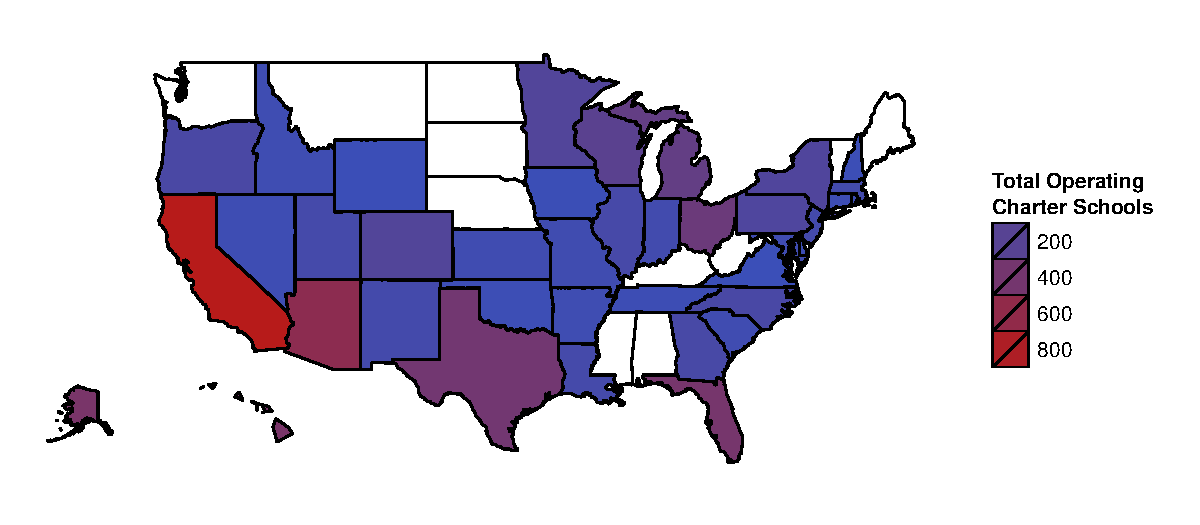
\includegraphics[width=\textwidth]{../Figures/CharterMapOperating.pdf}
\caption{Thematic Map of Number of Operating Charter Schools by State in 2009}
\label{fig:charterMap}
\end{figure}

\begin{figure}[h!]
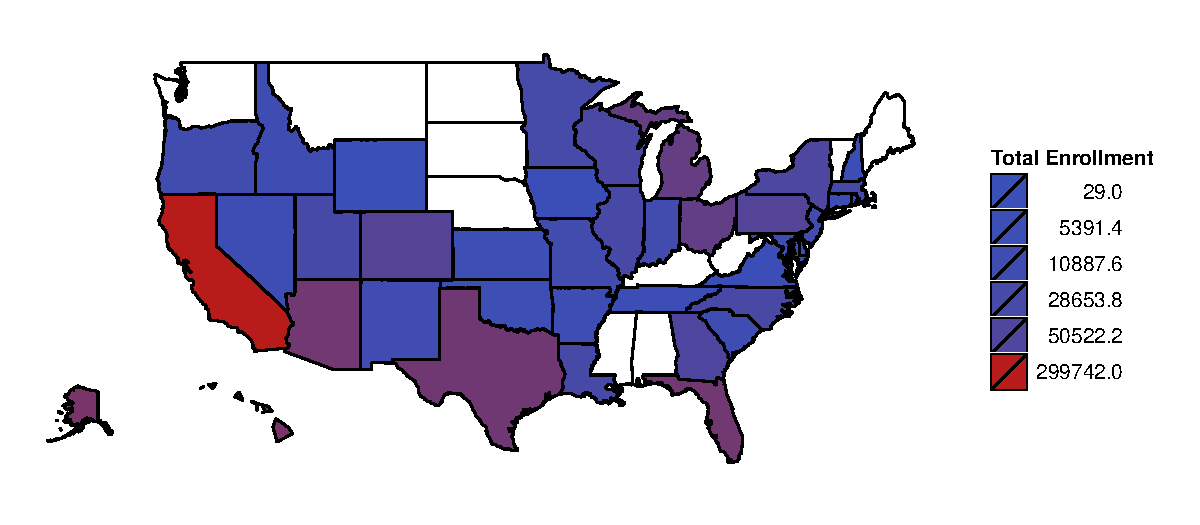
\includegraphics[width=\textwidth]{../Figures/CharterMapEnrollment.pdf}
\caption{Thematic Map of Charter School Enrollments by State in 2009}
\label{fig:charterMap}
\end{figure}

%==================== Appendix C ====================================================================
\newpage
\addcontentsline{toc}{subsection}{Appendix C: Student Background Questionnaire}
\subsection*{Appendix C\\NAEP Student Background Questionnaire}
\label{appendixQuestionnaire}
\subsubsection{Core Questions}
\begin{singlespace}
\begin{itemize}
	\item Are you Hispanic or Latino? [No, I am not Hispanic or Latino; Yes, I am Mexican, Mexican American, or Chicano; Yes, I am Puerto Rican or Puerto Rican American; Yes, I am Cuban or Cuban American; Yes, I am from some other Hispanic or Latino background]
	\item Which of the following best describes you? [White; Black or African American; Asian; American Indian or Alaska Native; Native Hawaiian or other Pacific Islander]
	\item Does your family get a newspaper at least four times a week?
	\item Does your family get any magazines regularly?
	\item About how many books are there in your home?
	\item Is there a computer at home that you use?
	\item Is there an encyclopedia in your home? It could be a set of books, or it could be on the computer.
	\item About how many pages a day do you have to read in school and for homework?
	\item How often do you talk about thinks you have studied in school with someone in your family?
	\item How many days were you absent from school in the last month?
	\item How far in school did your mother go? [Grade 8 Only]
	\item How far in school did your father go? [Grade 8 Only]
	\item How often do people in your home talk to each other in language other than English?
\end{itemize}
\end{singlespace}

\subsubsection{Grade 4 Math Related Questions}
\begin{singlespace}
\begin{itemize}
	\item Use computer at school for math
	\item Use computer to practice or drill on math
	\item Use computer to play math games
	\item Kind of calculator you normally use
	\item Use calculator for math tests-student
	\item Difficulty of this math test
	\item Effort on this math test
	\item Importance of success on this math test
	\item The math work is too hard
	\item I have done a good job on my homework
	\item I have done a good job in class
	\item The math work is too easy
	\item I like what we do in math class
\end{itemize}
\end{singlespace}

\subsubsection{Grade 4 Reading Related Questions}
\begin{singlespace}
\begin{itemize}
	\item Learn a lot when reading books
	\item Reading is a favorite activity
	\item Writing stories or letters is a favorite activity
	\item Writing helps share ideas
	\item Read for fun on own
	\item Talk with friends about what you read
	\item Write e-mails to friends or family
	\item Read stories or poems for fun
	\item Read to learn about real things
	\item Read stories on Internet for fun
	\item Class discussion about something class has read
	\item Work in groups to talk about something read
	\item Write in journal about something read
	\item Write a book report
	\item Make presentation to class about something read
	\item Do school project about something read
	\item Read books or magazines for reading
	\item Read books or magazines for science
	\item Read books or magazines for social studies/history
	\item Read books or magazines for math
	\item Write long answers on reading tests
	\item Read own books for reading assignment
	\item Difficulty of this reading test
	\item Effort on this reading test
	\item Importance of success on this reading test
\end{itemize}
\end{singlespace}

\subsubsection{Grade 8 Math Related Questions}
\begin{singlespace}
\begin{itemize}
	\item Use computer at school for math
	\item Use computer to practice or drill on math
	\item Use computer to play math games
	\item Kind of calculator you normally use
	\item Use calculator for math tests-student
	\item Difficulty of this math test
	\item Effort on this math test
	\item Importance of success on this math test
	\item Time per day on computer for math work
	\item Use spreadsheet program for math assignments
	\item Use program to drill on math facts
	\item Use program for new lessons on problem-solving
	\item Use Internet to learn things for math class
	\item Use calculator program for math class
	\item Using graphing program for charts for math class
	\item Use statistical program for math class
	\item Use word processing program for math class
	\item Use drawing program for math class
	\item Use basic four-function calculator in math class
	\item Use scientific calculator in math class
	\item Use graphing calculator in math class
	\item Have clear understanding what teacher asking to do
	\item The math work is too easy
	\item The math work is boring
	\item I have done a good job on my homework
	\item I have done a good job on my classwork
	\item The math work is challenging
	\item The math work is engaging and interesting
	\item I am learning
\end{itemize}
\end{singlespace}

\subsubsection{Grade 8 Reading Related Questions}
\begin{singlespace}
\begin{itemize}
	\item Write long answers on reading tests
	\item Learn a lot when reading books
	\item Reading is a favorite activity
	\item Writing stories or letters is a favorite activity
	\item Writing helps share ideas
	\item Read for fun on own
	\item Talk with friends about what you read
	\item Write e-mails to friends or family
	\item Read comic books or joke books outside school
	\item Read fiction books or stories outside school
	\item Read plays outside school
	\item Read poems outside school
	\item Read biographies/autobiographies outside school
	\item Read books on science outside school
	\item Read books on technology outside school
	\item Read books on other countries outside school
	\item Read books on history outside school
	\item Read other non-fiction books outside school
	\item Read newspaper articles or stories outside school
	\item Read magazine articles or stories outside school
	\item Read Internet articles or stories outside school
	\item Class discussion about something class has read
	\item Work in groups to talk about something read
	\item Write in journal about something read
	\item Write report or paper about something read
	\item Make presentation to class about something read
	\item Done project about something read
	\item Read other than textbook for English class
	\item Read other than textbook for science class
	\item Read other than textbook for social studies class
	\item Read other than textbook for math class
	\item Explain understanding of what you read
	\item Discuss interpretation of what you read
	\item Difficulty of this reading test
	\item Effort on this reading test
	\item Importance of success on this reading test
\end{itemize}
\end{singlespace}

%==================== Appendix D ====================================================================
\newpage
\addcontentsline{toc}{subsection}{Appendix D: Descriptive Statistics}
\subsection*{Appendix D\\Descriptive Statistics}
\label{appendixDescriptives}

\begin{singlespace}

% latex table generated in R 2.13.0 by xtable 1.5-6 package
% Thu Jun  2 18:56:20 2011
\begin{longtable}{lrrrr}
\caption{Descriptive Statistics: Grade 4 Math Student Variables} \\ 
   \thickline & \multicolumn{2}{c}{Public Schools} & \multicolumn{2}{c}{Charter Schools} \\ \endfirsthead \multicolumn{5}{l}{{...continued from previous page}}\\ \hline & \multicolumn{2}{c}{Charter Schools} & \multicolumn{2}{c}{Public Schools}  \\ \hline \endhead \hline & \multicolumn{4}{c}{gender} \\ \cline{2-5} Male & 72662 & 51\% & 1681 & 50\% \\ 
  Female & 70622 & 49\% & 1666 & 50\% \\ 
  Unknown &  35 & 0\% &   0 & 0\% \\ 
   \hline & \multicolumn{4}{c}{race} \\ \cline{2-5} White & 78078 & 54\% & 1207 & 36\% \\ 
  Black & 24605 & 17\% & 1376 & 41\% \\ 
  Hispanic & 28206 & 20\% & 577 & 17\% \\ 
  Asian American & 7515 & 5\% &  96 & 3\% \\ 
  American Indian & 3108 & 2\% &  47 & 1\% \\ 
  Other & 1807 & 1\% &  44 & 1\% \\ 
  Unknown &   0 & 0\% &   0 & 0\% \\ 
   \hline & \multicolumn{4}{c}{iep} \\ \cline{2-5} Yes & 16607 & 12\% & 311 & 9\% \\ 
  No & 126697 & 88\% & 3036 & 91\% \\ 
  Unknown &  15 & 0\% &   0 & 0\% \\ 
   \hline & \multicolumn{4}{c}{ell} \\ \cline{2-5} Yes & 16091 & 11\% & 252 & 8\% \\ 
  No & 127200 & 89\% & 3095 & 92\% \\ 
  Unknown &  28 & 0\% &   0 & 0\% \\ 
   \hline & \multicolumn{4}{c}{lunch} \\ \cline{2-5} Not eligible & 74755 & 52\% & 1393 & 42\% \\ 
  Reduced & 9728 & 7\% & 197 & 6\% \\ 
  Free & 57825 & 40\% & 1582 & 47\% \\ 
  Unknown & 1011 & 1\% & 175 & 5\% \\ 
   \hline & \multicolumn{4}{c}{books} \\ \cline{2-5} 0-10 & 17170 & 12\% & 405 & 12\% \\ 
  11-25 & 30527 & 21\% & 684 & 20\% \\ 
  26-100 & 46980 & 33\% & 1061 & 32\% \\ 
  $>$100 & 45043 & 31\% & 1083 & 32\% \\ 
  Unknown & 3599 & 3\% & 114 & 3\% \\ 
   \hline & \multicolumn{4}{c}{birthyear} \\ \cline{2-5} 1993 &  40 & 0\% &   0 & 0\% \\ 
  1994 & 289 & 0\% &   7 & 0\% \\ 
  1995 & 3914 & 3\% &  70 & 2\% \\ 
  1996 & 51306 & 36\% & 1033 & 31\% \\ 
  1997 & 87408 & 61\% & 2205 & 66\% \\ 
  1998 & 251 & 0\% &  29 & 1\% \\ 
  1999 & 108 & 0\% &   3 & 0\% \\ 
  2000 &   3 & 0\% &   0 & 0\% \\ 
  Unknown &   0 & 0\% &   0 & 0\% \\ 
   \hline & \multicolumn{4}{c}{newspapers} \\ \cline{2-5} yes & 44064 & 31\% & 1003 & 30\% \\ 
  no & 46298 & 32\% & 1143 & 34\% \\ 
  Unknown & 52957 & 37\% & 1201 & 36\% \\ 
   \hline & \multicolumn{4}{c}{magazines} \\ \cline{2-5} yes & 84482 & 59\% & 1930 & 58\% \\ 
  no & 31141 & 22\% & 701 & 21\% \\ 
  Unknown & 27696 & 19\% & 716 & 21\% \\ 
   \hline & \multicolumn{4}{c}{computer} \\ \cline{2-5} yes & 119361 & 83\% & 2810 & 84\% \\ 
  no & 19877 & 14\% & 411 & 12\% \\ 
  Unknown & 4081 & 3\% & 126 & 4\% \\ 
   \hline & \multicolumn{4}{c}{encyclopedia} \\ \cline{2-5} yes & 72434 & 51\% & 1761 & 53\% \\ 
  no & 23257 & 16\% & 490 & 15\% \\ 
  Unknown & 47628 & 33\% & 1096 & 33\% \\ 
   \hline & \multicolumn{4}{c}{pagesread} \\ \cline{2-5} $<$5 & 29967 & 21\% & 800 & 24\% \\ 
  5-10 & 26429 & 18\% & 678 & 20\% \\ 
  11-15 & 19560 & 14\% & 449 & 13\% \\ 
  16-20 & 20369 & 14\% & 447 & 13\% \\ 
  $>$20 & 43341 & 30\% & 858 & 26\% \\ 
  Unknown & 3653 & 3\% & 115 & 3\% \\ 
   \hline & \multicolumn{4}{c}{talkstudies} \\ \cline{2-5} Never & 25156 & 18\% & 604 & 18\% \\ 
  1-2 per month & 18463 & 13\% & 431 & 13\% \\ 
  1 per week & 16051 & 11\% & 359 & 11\% \\ 
  2-3 times per week & 28174 & 20\% & 553 & 17\% \\ 
  Every day & 51862 & 36\% & 1288 & 38\% \\ 
  Unknown & 3613 & 3\% & 112 & 3\% \\ 
   \hline & \multicolumn{4}{c}{daysabsent} \\ \cline{2-5} None & 69196 & 48\% & 1504 & 45\% \\ 
  1-2 & 42220 & 29\% & 949 & 28\% \\ 
  3-4 & 17372 & 12\% & 461 & 14\% \\ 
  5-10 & 7004 & 5\% & 174 & 5\% \\ 
  $>$10 & 3943 & 3\% & 149 & 4\% \\ 
  Unknown & 3584 & 3\% & 110 & 3\% \\ 
   \hline & \multicolumn{4}{c}{langinhome} \\ \cline{2-5} Never & 71636 & 50\% & 1569 & 47\% \\ 
  Once in a while & 31552 & 22\% & 785 & 23\% \\ 
  Half the time & 10935 & 8\% & 296 & 9\% \\ 
  All or most of the time & 25557 & 18\% & 588 & 18\% \\ 
  Unknown & 3639 & 3\% & 109 & 3\% \\ 
  \hline
\label{g4mathstudent}
\end{longtable}
 \clearpage
% latex table generated in R 2.13.0 by xtable 1.5-6 package
% Thu Jun  2 19:08:03 2011
\begin{sidewaystable}[htb]
\begin{center}
\caption{Descriptive Statistics: Grade 4 Math Scores by State}
\label{g4mathdesc}
{\smaller
\begin{tabular}{lrrrrrr@{\extracolsep{10pt}}rrrrrr}
  \hline & \multicolumn{6}{c}{Charter Schools} & \multicolumn{6}{c}{Public Schools} \\ \cline{2-7} \cline{8-13} & n & mean & sd & median & min & max & n & mean & sd & median & min & max \\ 
  \hline
Overall & 3347 & 233.09 & 28.81 & 234.25 & 127.15 & 313.10 & 143319 & 238.04 & 27.94 & 239.86 & 105.92 & 336.74 \\ 
  Alaska &  96 & 248.66 & 28.59 & 252.18 & 171.68 & 310.14 & 2861 & 238.77 & 28.86 & 241.24 & 132.44 & 315.60 \\ 
  Arizona & 244 & 233.47 & 28.73 & 235.46 & 127.15 & 296.09 & 3294 & 231.87 & 30.99 & 233.85 & 105.92 & 327.46 \\ 
  Arkansas &  20 & 245.97 & 21.14 & 248.87 & 196.54 & 276.03 & 3087 & 237.70 & 26.85 & 239.32 & 134.61 & 305.83 \\ 
  California & 276 & 226.95 & 29.27 & 228.80 & 160.57 & 296.81 & 9602 & 227.17 & 31.72 & 228.37 & 114.90 & 327.37 \\ 
  Colorado & 176 & 251.14 & 24.70 & 254.54 & 173.59 & 303.78 & 3195 & 239.46 & 28.61 & 241.33 & 117.05 & 322.84 \\ 
  Connecticut &   9 & 241.58 & 20.00 & 238.28 & 218.62 & 275.62 & 3198 & 243.22 & 28.31 & 245.82 & 108.81 & 325.12 \\ 
  Delaware & 186 & 237.21 & 20.66 & 238.58 & 180.13 & 290.34 & 3111 & 242.21 & 23.41 & 242.86 & 161.25 & 313.35 \\ 
  Dist. of Columbia & 376 & 214.20 & 27.89 & 215.33 & 132.74 & 294.06 & 1560 & 213.79 & 31.95 & 212.67 & 124.08 & 316.65 \\ 
  Florida & 216 & 248.04 & 20.56 & 249.88 & 193.11 & 288.81 & 4971 & 241.68 & 24.92 & 242.52 & 138.45 & 317.76 \\ 
  Georgia &  81 & 229.24 & 24.25 & 230.31 & 166.06 & 281.96 & 4667 & 231.41 & 27.24 & 231.09 & 128.42 & 322.00 \\ 
  Hawaii &  79 & 242.36 & 19.99 & 244.03 & 186.62 & 291.17 & 3364 & 234.29 & 30.00 & 236.98 & 118.25 & 316.46 \\ 
  Idaho & 120 & 257.56 & 23.91 & 260.58 & 184.00 & 297.52 & 3464 & 240.54 & 25.65 & 242.24 & 145.46 & 310.83 \\ 
  Illinois &  91 & 224.57 & 19.50 & 223.46 & 181.67 & 271.27 & 4782 & 231.36 & 29.82 & 231.94 & 121.28 & 316.82 \\ 
  Indiana &   9 & 193.44 & 19.40 & 194.96 & 152.18 & 213.88 & 3131 & 245.59 & 25.00 & 247.08 & 120.78 & 336.74 \\ 
  Iowa &   4 & 230.07 & 18.44 & 226.29 & 212.35 & 255.36 & 3023 & 242.76 & 24.99 & 244.53 & 120.93 & 315.95 \\ 
  Louisiana & 157 & 236.79 & 25.71 & 236.10 & 178.70 & 295.55 & 2886 & 230.26 & 25.13 & 230.64 & 142.70 & 302.89 \\ 
  Maryland &  22 & 214.61 & 19.49 & 217.25 & 158.19 & 257.62 & 3570 & 240.68 & 29.14 & 241.44 & 153.03 & 326.72 \\ 
  Massachusetts &  58 & 232.12 & 20.78 & 232.36 & 182.92 & 279.23 & 4084 & 246.74 & 26.09 & 248.13 & 149.06 & 320.80 \\ 
  Michigan & 342 & 225.82 & 28.71 & 225.91 & 148.98 & 298.83 & 2995 & 239.41 & 27.63 & 242.01 & 134.29 & 316.89 \\ 
  Minnesota &  33 & 250.06 & 23.79 & 249.35 & 202.82 & 304.24 & 3538 & 246.26 & 26.83 & 248.77 & 116.79 & 317.13 \\ 
  Missouri &  29 & 202.01 & 25.97 & 200.61 & 147.55 & 255.00 & 3168 & 240.12 & 26.02 & 241.56 & 146.54 & 318.74 \\ 
  Nevada &  28 & 226.90 & 28.63 & 233.98 & 147.17 & 270.87 & 4005 & 231.03 & 28.32 & 233.32 & 130.20 & 312.34 \\ 
  New Hampshire &   5 & 244.07 & 12.22 & 246.95 & 227.90 & 258.95 & 3343 & 248.51 & 23.91 & 250.00 & 147.79 & 324.29 \\ 
  New Jersey &  34 & 225.05 & 20.64 & 221.87 & 178.65 & 264.08 & 3306 & 248.15 & 25.70 & 249.85 & 157.81 & 321.31 \\ 
  New Mexico &   3 & 173.61 & 6.41 & 171.26 & 168.71 & 180.86 & 3149 & 228.02 & 27.68 & 229.53 & 126.99 & 310.59 \\ 
  New York &  20 & 233.30 & 16.80 & 231.55 & 203.43 & 263.35 & 4568 & 240.78 & 27.02 & 242.46 & 122.86 & 331.88 \\ 
  North Carolina &  78 & 257.74 & 22.52 & 259.24 & 187.51 & 292.10 & 5480 & 240.30 & 26.37 & 240.93 & 124.66 & 319.32 \\ 
  Ohio & 122 & 223.41 & 22.45 & 225.62 & 166.82 & 268.12 & 3720 & 237.86 & 28.20 & 239.37 & 120.25 & 311.48 \\ 
  Oklahoma &   5 & 197.63 & 18.58 & 192.62 & 178.83 & 218.80 & 3220 & 237.31 & 23.71 & 238.55 & 124.41 & 311.19 \\ 
  Oregon &  14 & 239.03 & 31.96 & 242.63 & 173.87 & 275.80 & 3486 & 235.54 & 27.50 & 237.30 & 127.15 & 314.33 \\ 
  Pennsylvania &  98 & 244.60 & 29.57 & 246.79 & 157.89 & 296.81 & 3381 & 244.27 & 27.55 & 247.56 & 126.32 & 321.62 \\ 
  Rhode Island &  30 & 230.02 & 25.71 & 225.69 & 177.33 & 293.88 & 3070 & 235.25 & 27.73 & 237.93 & 129.90 & 303.57 \\ 
  South Carolina &   7 & 233.80 & 24.04 & 243.01 & 203.14 & 269.53 & 3560 & 237.56 & 28.14 & 239.44 & 115.53 & 316.96 \\ 
  Tennessee &   9 & 211.69 & 17.60 & 213.20 & 187.58 & 240.25 & 3237 & 233.45 & 26.21 & 235.39 & 115.24 & 311.24 \\ 
  Texas & 129 & 220.51 & 22.42 & 218.67 & 164.33 & 278.31 & 8746 & 239.69 & 24.51 & 239.55 & 128.55 & 314.11 \\ 
  Utah &  76 & 249.71 & 25.83 & 255.54 & 183.80 & 294.22 & 3618 & 239.43 & 26.44 & 242.26 & 126.79 & 308.68 \\ 
  Wisconsin &  57 & 220.93 & 30.40 & 211.70 & 153.62 & 290.65 & 3170 & 245.18 & 26.60 & 248.06 & 148.39 & 319.55 \\ 
  Wyoming &   8 & 274.94 & 23.59 & 277.09 & 244.79 & 313.10 & 2709 & 243.88 & 23.41 & 245.60 & 145.86 & 318.65 \\ 
   \hline
\end{tabular}
}
\end{center}
\end{sidewaystable}
 \clearpage
\end{singlespace}

\begin{figure}[h]
\begin{center}
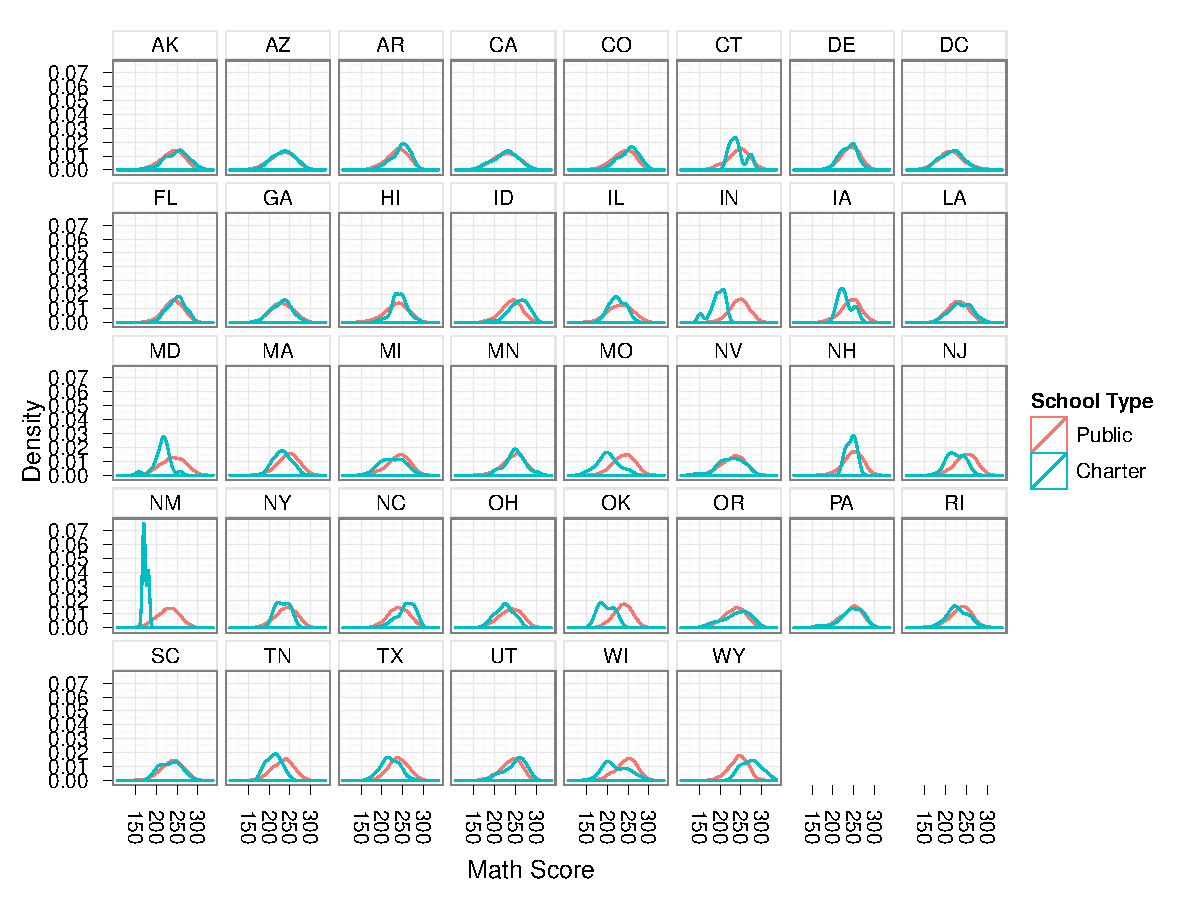
\includegraphics[width=\textwidth,angle=90]{../Figures/g4mathDensityByState.pdf}
\caption{Density Distribution of Grade 4 Math Scores by State}
\label{fig:g4math:density}
\end{center}
\end{figure}
\clearpage


%==================== Appendix E ====================================================================
\cleardoublepage
\addcontentsline{toc}{subsection}{Appendix E: Covariate Missingness}
\subsection*{Appendix E\\Covariate Missingness}
\label{appendixmissing}

\begin{figure}[h]
\begin{center}
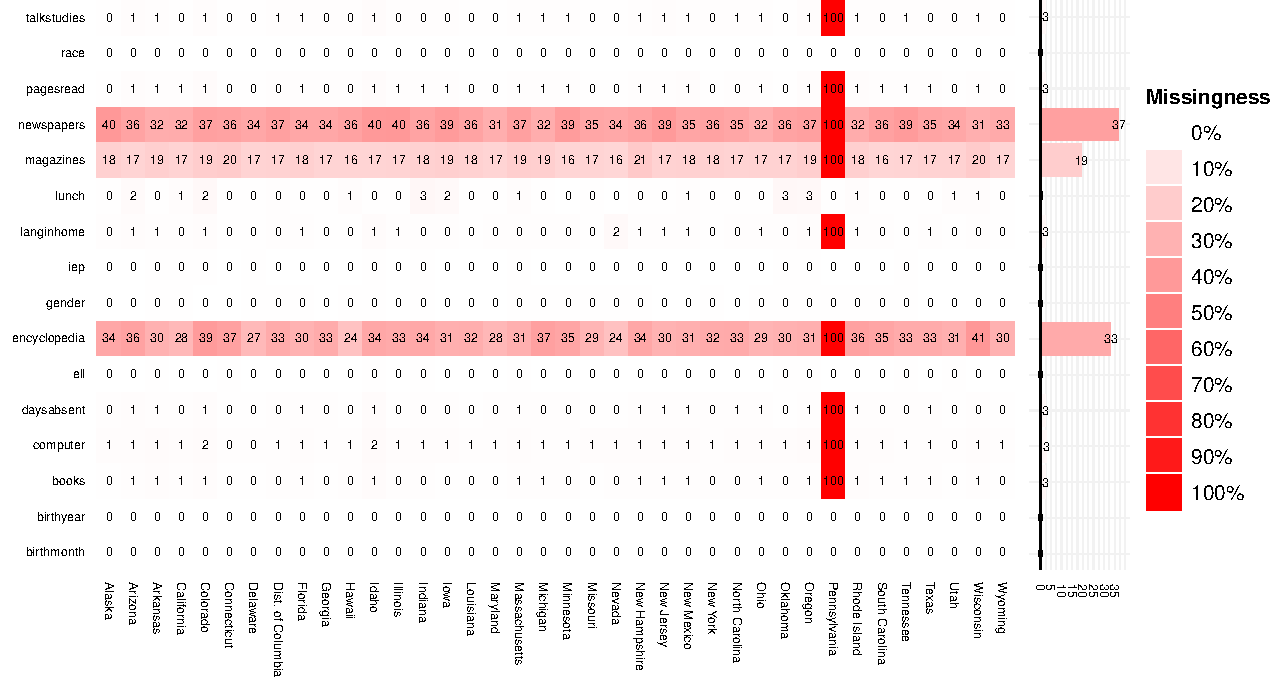
\includegraphics[width=\textwidth]{../Figures/g4mathmissing.pdf}
\caption{Covariate Missingness for Grade 4 Math}
\label{fig:g4math:missing}
\end{center}
\end{figure}


%==================== Appendix F ====================================================================
\cleardoublepage
\addcontentsline{toc}{subsection}{Appendix F: Logistic Regression Full Model Results}
\subsection*{Appendix F\\Logistic Regression Full Model}
\label{appendixlogistic}
\begin{singlespace}
% latex table generated in R 2.13.0 by xtable 1.5-6 package
% Sun Jun 26 16:53:32 2011
\begin{longtable}{lrrr@{\extracolsep{10pt}}rrrr}
\caption{Logistic Regression Level 1 Summary: Grade 4 math} \\ 
  \hline
  & \multicolumn{3}{c}{Charter Schools} & \multicolumn{3}{c}{Public Schools} & \\ \cline{2-4} \cline{5-7} State & n & Score & SE & n & Score & SE & Diff \\ \endfirsthead \multicolumn{8}{l}{{...continued from previous page}}\\ \hline & \multicolumn{3}{c}{Charter Schools} & \multicolumn{3}{c}{Public Schools} & \\ \cline{2-4} \cline{5-7} State & n & Score & SE & n & Score & SE & Diff \\ \hline \endhead \hline \endfoot \endlastfoot \hline
Alaska &   7 & 251.69 & 12.92 & 989 & 230.40 & 0.91 & 21.30 \\ 
  Alaska &  11 & 243.73 & 11.19 & 567 & 234.07 & 1.24 & 9.66 \\ 
  Alaska &  78 & 249.08 & 3.07 & 1096 & 251.09 & 0.73 & -2.01 \\ 
  Arizona &  20 & 218.25 & 4.99 & 794 & 224.32 & 1.17 & -6.07 \\ 
  Arizona & 222 & 234.86 & 1.94 & 2381 & 235.32 & 0.60 & -0.46 \\ 
  Arkansas &   4 & 241.24 & 15.43 & 433 & 253.39 & 0.94 & -12.15 \\ 
  Arkansas &   4 & 252.13 & 8.36 & 193 & 253.01 & 1.62 & -0.88 \\ 
  Arkansas &  12 & 245.50 & 5.87 & 133 & 249.91 & 2.13 & -4.41 \\ 
  California &  10 & 221.76 & 9.11 & 827 & 222.99 & 1.22 & -1.23 \\ 
  California & 165 & 227.95 & 2.39 & 6695 & 229.10 & 0.39 & -1.15 \\ 
  California & 101 & 225.82 & 2.69 & 2080 & 222.62 & 0.64 & 3.20 \\ 
  Colorado &  32 & 240.62 & 5.31 & 918 & 228.89 & 0.92 & 11.72 \\ 
  Colorado & 144 & 253.48 & 1.90 & 2150 & 245.43 & 0.58 & 8.05 \\ 
  Connecticut &   6 & 245.19 & 9.24 &  55 & 227.68 & 3.17 & 17.52 \\ 
  Delaware &  40 & 248.90 & 2.78 & 1165 & 248.66 & 0.65 & 0.24 \\ 
  Delaware & 145 & 233.93 & 1.69 & 1727 & 238.87 & 0.56 & -4.93 \\ 
  Dist. of Columbia & 376 & 214.20 & 1.44 & 1555 & 213.74 & 0.81 & 0.46 \\ 
  Florida &   6 & 229.13 & 5.84 & 695 & 226.66 & 0.97 & 2.47 \\ 
  Florida &  45 & 239.46 & 3.04 & 2031 & 239.53 & 0.55 & -0.07 \\ 
  Florida & 165 & 251.07 & 1.54 & 2241 & 248.32 & 0.47 & 2.75 \\ 
  Georgia &  19 & 235.92 & 7.36 & 2349 & 235.12 & 0.58 & 0.80 \\ 
  Georgia &  27 & 229.93 & 4.38 & 1317 & 229.37 & 0.72 & 0.56 \\ 
  Georgia &  35 & 225.07 & 3.38 & 539 & 225.12 & 1.08 & -0.05 \\ 
  Hawaii &   9 & 233.92 & 8.54 & 1254 & 229.08 & 0.82 & 4.84 \\ 
  Hawaii &  15 & 246.91 & 6.30 & 929 & 238.42 & 0.92 & 8.49 \\ 
  Hawaii &  54 & 243.32 & 2.26 & 757 & 247.66 & 0.99 & -4.34 \\ 
  Idaho &  28 & 256.70 & 4.19 & 1130 & 243.43 & 0.70 & 13.27 \\ 
  Idaho &  89 & 258.91 & 2.50 & 1275 & 249.12 & 0.64 & 9.79 \\ 
  Illinois &   6 & 221.80 & 8.61 & 604 & 220.57 & 1.20 & 1.22 \\ 
  Illinois &  24 & 219.03 & 4.76 & 1133 & 219.02 & 0.78 & 0.01 \\ 
  Illinois &  60 & 226.93 & 2.27 & 891 & 214.41 & 0.78 & 12.51 \\ 
  Indiana &   7 & 192.21 & 8.25 &  56 & 220.26 & 3.24 & -28.05 \\ 
  Iowa &   4 & 230.07 & 9.22 &  17 & 240.43 & 6.29 & -10.35 \\ 
  Louisiana &   5 & 247.46 & 10.87 & 589 & 235.04 & 0.96 & 12.41 \\ 
  Louisiana &  18 & 235.47 & 5.20 & 878 & 234.11 & 0.84 & 1.36 \\ 
  Louisiana & 134 & 236.57 & 2.27 & 1382 & 225.71 & 0.68 & 10.85 \\ 
  Maryland &   4 & 215.36 & 5.68 & 678 & 234.03 & 1.05 & -18.67 \\ 
  Maryland &   8 & 215.15 & 5.48 & 336 & 226.60 & 1.49 & -11.45 \\ 
  Maryland &   9 & 212.58 & 8.93 & 151 & 223.72 & 2.13 & -11.15 \\ 
  Massachusetts &   7 & 246.67 & 11.07 & 1325 & 247.03 & 0.73 & -0.37 \\ 
  Massachusetts &  10 & 225.57 & 7.55 & 392 & 235.81 & 1.29 & -10.24 \\ 
  Massachusetts &  39 & 231.15 & 2.64 & 392 & 234.89 & 1.05 & -3.75 \\ 
  Michigan &  14 & 249.97 & 7.42 & 520 & 248.99 & 1.00 & 0.98 \\ 
  Michigan & 328 & 224.79 & 1.56 & 2420 & 237.49 & 0.57 & -12.70 \\ 
  Minnesota &  11 & 253.55 & 8.34 & 1882 & 249.77 & 0.59 & 3.78 \\ 
  Minnesota &  13 & 250.22 & 7.21 & 482 & 244.53 & 1.25 & 5.69 \\ 
  Minnesota &   9 & 245.57 & 5.31 & 152 & 239.14 & 2.30 & 6.43 \\ 
  Missouri &  26 & 199.23 & 4.90 & 161 & 219.72 & 1.77 & -20.48 \\ 
  Nevada &   9 & 224.35 & 8.06 & 1709 & 230.26 & 0.70 & -5.90 \\ 
  Nevada &  12 & 226.30 & 10.06 & 457 & 234.81 & 1.26 & -8.51 \\ 
  Nevada &   6 & 236.05 & 9.83 & 117 & 230.32 & 2.64 & 5.72 \\ 
  New Jersey &   4 & 234.57 & 9.00 & 348 & 234.79 & 1.32 & -0.22 \\ 
  New Jersey &   7 & 229.02 & 9.25 & 419 & 236.38 & 1.18 & -7.36 \\ 
  New Jersey &  23 & 222.19 & 4.18 & 308 & 236.33 & 1.28 & -14.15 \\ 
  New York &   5 & 232.09 & 7.25 & 266 & 230.84 & 1.46 & 1.25 \\ 
  New York &  11 & 232.49 & 5.37 & 142 & 231.51 & 1.87 & 0.98 \\ 
  North Carolina &  13 & 245.21 & 7.59 & 1626 & 240.31 & 0.64 & 4.90 \\ 
  North Carolina &  14 & 256.95 & 6.68 & 965 & 255.17 & 0.77 & 1.78 \\ 
  North Carolina &  49 & 261.52 & 2.78 & 594 & 253.26 & 0.86 & 8.26 \\ 
  Ohio &  14 & 240.94 & 5.13 & 1636 & 250.50 & 0.58 & -9.56 \\ 
  Ohio &  27 & 232.63 & 4.05 & 1012 & 237.13 & 0.80 & -4.50 \\ 
  Ohio &  81 & 217.31 & 2.33 & 1011 & 217.09 & 0.81 & 0.22 \\ 
  Oregon &   7 & 228.47 & 13.59 &  54 & 230.51 & 3.66 & -2.05 \\ 
  Pennsylvania &   4 & 228.45 & 6.72 & 623 & 239.89 & 1.08 & -11.43 \\ 
  Pennsylvania &  48 & 245.15 & 4.33 & 1681 & 247.83 & 0.67 & -2.69 \\ 
  Pennsylvania &  46 & 245.44 & 4.45 & 840 & 242.79 & 0.97 & 2.65 \\ 
  Rhode Island &   9 & 243.08 & 9.24 & 1593 & 241.33 & 0.62 & 1.75 \\ 
  Rhode Island &   4 & 236.79 & 10.48 & 280 & 235.65 & 1.73 & 1.14 \\ 
  Rhode Island &  15 & 220.68 & 5.10 & 129 & 217.75 & 2.98 & 2.94 \\ 
  Tennessee &   4 & 206.64 & 8.92 &  74 & 219.33 & 3.04 & -12.70 \\ 
  Tennessee &   5 & 215.73 & 8.19 &  73 & 216.15 & 3.05 & -0.43 \\ 
  Texas &  19 & 225.34 & 5.12 & 3172 & 239.87 & 0.42 & -14.53 \\ 
  Texas &  37 & 229.58 & 3.86 & 1536 & 235.41 & 0.54 & -5.83 \\ 
  Texas &  70 & 214.56 & 2.47 & 1075 & 226.00 & 0.65 & -11.44 \\ 
  Utah &  12 & 249.95 & 7.67 & 977 & 239.68 & 0.81 & 10.26 \\ 
  Utah &  28 & 254.61 & 4.43 & 1618 & 243.56 & 0.61 & 11.05 \\ 
  Utah &  36 & 245.81 & 4.56 & 530 & 244.48 & 1.09 & 1.33 \\ 
  Wisconsin &  12 & 256.87 & 5.12 & 1952 & 251.29 & 0.53 & 5.58 \\ 
  Wisconsin &   6 & 242.42 & 11.78 & 290 & 235.29 & 1.69 & 7.13 \\ 
  Wisconsin &  38 & 206.92 & 3.54 & 297 & 219.07 & 1.61 & -12.16 \\ 
   \hline
\hline
\label{g4mathlrlevel1}
\end{longtable}
 \clearpage
% latex table generated in R 2.13.0 by xtable 1.5-6 package
% Sun Jun 26 16:53:32 2011
\begin{table}[ht]
\begin{center}
\caption{Logistic RegressionLevel 2 Summary: Grade 4 math}
\label{g4mathlrlevel2}
\begin{tabular}{lrrrrrr}
  \hline
  State & n & Public & Charter & Diff & \multicolumn{2}{c}{Confidence Interval} \\ \hline
Alaska & 2748 & 240.01 & 248.90 & 8.89 & -2.52 & 20.29 \\ 
  Arizona & 3417 & 232.70 & 230.91 & -1.79 & -7.20 & 3.61 \\ 
  Arkansas & 779 & 252.65 & 244.79 & -7.86 & -20.11 & 4.39 \\ 
  California & 9878 & 227.15 & 226.96 & -0.20 & -6.67 & 6.27 \\ 
  Colorado & 3244 & 240.59 & 249.71 & 9.12 & 3.49 & 14.76 \\ 
  Connecticut &  61 & 227.68 & 245.19 & 17.52 & -2.04 & 37.07 \\ 
  Delaware & 3077 & 242.70 & 239.80 & -2.91 & -6.20 & 0.39 \\ 
  Dist. of Columbia & 1931 & 213.74 & 214.20 & 0.46 & -2.78 & 3.70 \\ 
  Florida & 5183 & 241.87 & 243.45 & 1.58 & -2.90 & 6.07 \\ 
  Georgia & 4286 & 231.98 & 232.59 & 0.61 & -5.48 & 6.70 \\ 
  Hawaii & 3018 & 236.99 & 240.51 & 3.52 & -3.65 & 10.68 \\ 
  Idaho & 2522 & 246.51 & 257.89 & 11.39 & 6.51 & 16.26 \\ 
  Illinois & 2718 & 217.76 & 222.41 & 4.65 & -2.03 & 11.34 \\ 
  Indiana &  63 & 220.26 & 192.21 & -28.05 & -45.77 & -10.33 \\ 
  Iowa &  21 & 240.43 & 230.07 & -10.35 & -33.72 & 13.01 \\ 
  Louisiana & 3006 & 230.06 & 238.39 & 8.33 & 0.26 & 16.40 \\ 
  Maryland & 1186 & 230.49 & 214.93 & -15.56 & -23.57 & -7.55 \\ 
  Massachusetts & 2165 & 242.53 & 239.66 & -2.87 & -11.88 & 6.13 \\ 
  Michigan & 3282 & 239.36 & 228.88 & -10.48 & -18.00 & -2.96 \\ 
  Minnesota & 2549 & 248.08 & 252.40 & 4.32 & -3.87 & 12.51 \\ 
  Missouri & 187 & 219.72 & 199.23 & -20.48 & -30.77 & -10.20 \\ 
  Nevada & 2310 & 231.19 & 225.37 & -5.81 & -16.59 & 4.97 \\ 
  New Jersey & 1109 & 235.86 & 228.74 & -7.12 & -16.11 & 1.87 \\ 
  New York & 424 & 231.08 & 232.23 & 1.15 & -8.02 & 10.32 \\ 
  North Carolina & 3261 & 247.33 & 251.95 & 4.63 & -2.28 & 11.54 \\ 
  Ohio & 3781 & 237.18 & 231.83 & -5.34 & -9.95 & -0.74 \\ 
  Oregon &  61 & 230.51 & 228.47 & -2.05 & -30.21 & 26.11 \\ 
  Pennsylvania & 3242 & 244.92 & 242.00 & -2.92 & -8.99 & 3.15 \\ 
  Rhode Island & 2030 & 238.86 & 240.61 & 1.75 & -8.24 & 11.74 \\ 
  Tennessee & 156 & 217.74 & 211.18 & -6.56 & -19.26 & 6.13 \\ 
  Texas & 5909 & 235.99 & 224.38 & -11.61 & -16.14 & -7.08 \\ 
  Utah & 3201 & 242.53 & 251.61 & 9.09 & 2.51 & 15.67 \\ 
  Wisconsin & 2595 & 245.31 & 248.77 & 3.47 & -5.38 & 12.31 \\ 
   \hline
\end{tabular}
\end{center}
\end{table}
 \clearpage
\end{singlespace}

%==================== Appendix G ====================================================================
\cleardoublepage
\addcontentsline{toc}{subsection}{Appendix G: Logistic Regression Step AIC Model Results}
\subsection*{Appendix G\\Logistic Regression Step AIC Model}
\label{appendixlogisticaic}
\begin{singlespace}
% latex table generated in R 2.13.0 by xtable 1.5-6 package
% Sun Jun 26 16:55:46 2011
\begin{longtable}{lrrr@{\extracolsep{10pt}}rrrr}
\caption{Logistic Regression Step AIC Level 1 Summary: Grade 4 math} \\ 
  \hline
  & \multicolumn{3}{c}{Charter Schools} & \multicolumn{3}{c}{Public Schools} & \\ \cline{2-4} \cline{5-7} State & n & Score & SE & n & Score & SE & Diff \\ \endfirsthead \multicolumn{8}{l}{{...continued from previous page}}\\ \hline & \multicolumn{3}{c}{Charter Schools} & \multicolumn{3}{c}{Public Schools} & \\ \cline{2-4} \cline{5-7} State & n & Score & SE & n & Score & SE & Diff \\ \hline \endhead \hline \endfoot \endlastfoot \hline
Alaska &   7 & 272.74 & 6.82 & 906 & 234.25 & 0.89 & 38.49 \\ 
  Alaska &   9 & 215.63 & 8.08 & 307 & 217.35 & 1.83 & -1.72 \\ 
  Alaska &  80 & 250.27 & 3.00 & 1311 & 251.15 & 0.64 & -0.88 \\ 
  Arizona &  20 & 214.02 & 6.33 & 638 & 222.31 & 1.29 & -8.29 \\ 
  Arizona & 223 & 235.33 & 1.89 & 2532 & 235.25 & 0.59 & 0.08 \\ 
  Arkansas &   4 & 253.75 & 12.04 & 466 & 250.11 & 0.98 & 3.64 \\ 
  Arkansas &   6 & 244.60 & 10.07 & 213 & 251.55 & 1.62 & -6.95 \\ 
  Arkansas &  10 & 243.69 & 6.15 & 147 & 252.48 & 1.90 & -8.79 \\ 
  California &   4 & 227.02 & 16.18 & 359 & 228.60 & 1.81 & -1.58 \\ 
  California & 224 & 227.28 & 1.99 & 8466 & 228.05 & 0.34 & -0.77 \\ 
  California &  48 & 225.40 & 3.94 & 777 & 216.94 & 1.03 & 8.45 \\ 
  Colorado &  26 & 239.33 & 6.17 & 948 & 224.26 & 0.88 & 15.08 \\ 
  Colorado & 150 & 253.19 & 1.87 & 2247 & 245.87 & 0.57 & 7.32 \\ 
  Connecticut &   6 & 238.97 & 6.96 &  97 & 222.65 & 2.60 & 16.32 \\ 
  Delaware &  36 & 251.54 & 2.85 & 1160 & 250.66 & 0.63 & 0.88 \\ 
  Delaware & 147 & 233.80 & 1.64 & 1763 & 237.81 & 0.55 & -4.01 \\ 
  Dist. of Columbia & 376 & 214.20 & 1.44 & 1557 & 213.76 & 0.81 & 0.44 \\ 
  Florida &   9 & 228.77 & 5.94 & 709 & 224.87 & 0.95 & 3.90 \\ 
  Florida &  38 & 236.09 & 3.05 & 1657 & 236.34 & 0.56 & -0.25 \\ 
  Florida & 169 & 251.76 & 1.50 & 2596 & 249.75 & 0.45 & 2.00 \\ 
  Georgia &  27 & 241.13 & 4.46 & 2457 & 236.60 & 0.57 & 4.54 \\ 
  Georgia &  22 & 227.31 & 5.59 & 1178 & 226.90 & 0.72 & 0.41 \\ 
  Georgia &  32 & 220.53 & 3.52 & 434 & 221.05 & 1.20 & -0.52 \\ 
  Hawaii &  12 & 238.35 & 8.01 & 1541 & 231.32 & 0.72 & 7.03 \\ 
  Hawaii &  16 & 247.12 & 6.07 & 539 & 238.34 & 1.30 & 8.78 \\ 
  Hawaii &  50 & 242.00 & 2.32 & 892 & 243.98 & 0.94 & -1.98 \\ 
  Idaho &  26 & 252.70 & 4.39 & 1006 & 242.82 & 0.75 & 9.88 \\ 
  Idaho &  91 & 259.04 & 2.53 & 1483 & 248.78 & 0.59 & 10.26 \\ 
  Illinois &   9 & 223.68 & 7.69 & 567 & 221.76 & 1.22 & 1.92 \\ 
  Illinois &  23 & 226.56 & 3.84 & 985 & 222.21 & 0.83 & 4.34 \\ 
  Illinois &  58 & 223.78 & 2.60 & 1060 & 211.21 & 0.72 & 12.57 \\ 
  Indiana &   7 & 192.21 & 8.25 &  84 & 217.71 & 2.48 & -25.50 \\ 
  Iowa &   4 & 230.07 & 9.22 & 503 & 229.18 & 1.12 & 0.89 \\ 
  Louisiana &   8 & 244.00 & 9.31 & 701 & 234.77 & 0.89 & 9.23 \\ 
  Louisiana &   9 & 238.24 & 8.52 & 709 & 232.97 & 0.96 & 5.27 \\ 
  Louisiana & 140 & 236.28 & 2.18 & 1430 & 226.68 & 0.67 & 9.60 \\ 
  Maryland &  11 & 212.37 & 8.02 & 960 & 234.03 & 0.94 & -21.66 \\ 
  Maryland &   8 & 213.64 & 2.95 & 389 & 223.28 & 1.30 & -9.64 \\ 
  Massachusetts &   8 & 245.06 & 8.83 & 976 & 244.91 & 0.89 & 0.16 \\ 
  Massachusetts &   8 & 217.83 & 6.85 & 289 & 235.81 & 1.53 & -17.97 \\ 
  Massachusetts &  39 & 231.15 & 2.64 & 440 & 235.02 & 0.96 & -3.88 \\ 
  Michigan &   5 & 248.24 & 21.54 & 146 & 239.40 & 1.94 & 8.84 \\ 
  Michigan & 337 & 225.49 & 1.54 & 2795 & 239.54 & 0.53 & -14.06 \\ 
  Minnesota &  22 & 246.47 & 5.02 & 1983 & 246.18 & 0.61 & 0.29 \\ 
  Minnesota &   8 & 266.15 & 6.17 & 307 & 258.52 & 1.33 & 7.63 \\ 
  Missouri &  25 & 198.28 & 5.00 & 184 & 218.69 & 1.73 & -20.41 \\ 
  Nevada &  13 & 221.33 & 5.70 & 1689 & 230.16 & 0.69 & -8.83 \\ 
  Nevada &   8 & 232.84 & 15.32 & 382 & 241.49 & 1.29 & -8.65 \\ 
  Nevada &   4 & 234.37 & 13.46 &  46 & 228.53 & 4.03 & 5.84 \\ 
  New Hampshire &   5 & 244.07 & 5.47 & 3343 & 248.51 & 0.41 & -4.43 \\ 
  New Jersey &   6 & 233.94 & 11.01 & 364 & 236.87 & 1.27 & -2.93 \\ 
  New Jersey &   4 & 215.92 & 7.53 & 328 & 235.46 & 1.34 & -19.54 \\ 
  New Jersey &  24 & 224.35 & 4.02 & 400 & 235.30 & 1.14 & -10.95 \\ 
  New York &   7 & 234.88 & 6.92 & 617 & 231.26 & 0.96 & 3.61 \\ 
  New York &   4 & 233.02 & 7.09 & 304 & 226.21 & 1.46 & 6.81 \\ 
  New York &   9 & 232.20 & 6.15 & 183 & 224.58 & 1.72 & 7.62 \\ 
  North Carolina &   5 & 251.62 & 10.95 & 2200 & 230.28 & 0.52 & 21.34 \\ 
  North Carolina &   9 & 239.19 & 8.35 & 1507 & 242.31 & 0.69 & -3.11 \\ 
  North Carolina &  20 & 257.05 & 5.68 & 988 & 254.82 & 0.72 & 2.23 \\ 
  North Carolina &  44 & 262.53 & 2.82 & 559 & 250.06 & 0.95 & 12.47 \\ 
  Ohio &  15 & 242.33 & 4.97 & 1794 & 249.86 & 0.55 & -7.54 \\ 
  Ohio &  25 & 229.49 & 4.12 & 790 & 236.36 & 0.93 & -6.87 \\ 
  Ohio &  82 & 218.10 & 2.36 & 1059 & 217.59 & 0.79 & 0.50 \\ 
  Oregon &   6 & 247.15 & 10.97 & 1431 & 237.94 & 0.66 & 9.20 \\ 
  Oregon &   6 & 221.30 & 13.66 &  50 & 223.67 & 4.01 & -2.37 \\ 
  Pennsylvania &   8 & 242.20 & 13.27 & 574 & 244.93 & 1.07 & -2.73 \\ 
  Pennsylvania &  53 & 247.42 & 3.65 & 1904 & 247.59 & 0.61 & -0.17 \\ 
  Pennsylvania &  37 & 241.08 & 5.30 & 671 & 237.16 & 1.20 & 3.92 \\ 
  Rhode Island &   9 & 233.66 & 11.11 & 1487 & 241.47 & 0.65 & -7.81 \\ 
  Rhode Island &  15 & 220.59 & 5.09 & 129 & 210.02 & 2.92 & 10.57 \\ 
  Tennessee &   5 & 214.32 & 9.31 & 208 & 219.68 & 1.60 & -5.36 \\ 
  Texas &   7 & 216.28 & 7.21 & 4304 & 243.17 & 0.40 & -26.89 \\ 
  Texas &  18 & 231.16 & 5.54 & 1984 & 243.33 & 0.48 & -12.17 \\ 
  Texas &  31 & 225.53 & 4.12 & 1302 & 235.24 & 0.58 & -9.71 \\ 
  Texas &  73 & 216.16 & 2.49 & 1156 & 225.47 & 0.64 & -9.30 \\ 
  Utah &  57 & 249.06 & 3.37 & 2596 & 243.25 & 0.49 & 5.80 \\ 
  Utah &  16 & 251.55 & 7.12 & 298 & 242.13 & 1.51 & 9.43 \\ 
  Wisconsin &  11 & 254.53 & 5.10 & 2001 & 252.46 & 0.52 & 2.07 \\ 
  Wisconsin &   4 & 252.19 & 13.46 & 352 & 238.03 & 1.34 & 14.16 \\ 
  Wisconsin &  39 & 206.80 & 3.45 & 303 & 218.11 & 1.65 & -11.31 \\ 
  Wyoming &   8 & 274.94 & 8.34 & 1188 & 250.35 & 0.62 & 24.59 \\ 
   \hline
\hline
\label{g4mathlraiclevel1}
\end{longtable}
 \clearpage
% latex table generated in R 2.13.0 by xtable 1.5-6 package
% Sun Jun 26 16:55:47 2011
\begin{table}[ht]
\begin{center}
\caption{Logistic Regression Step AIC Level 2 Summary: Grade 4 math}
\label{g4mathlraiclevel2}
\begin{tabular}{lrrrrrr}
  \hline
  State & n & Public & Charter & Diff & \multicolumn{2}{c}{Confidence Interval} \\ \hline
Alaska & 2620 & 241.19 & 253.92 & 12.73 & 5.41 & 20.06 \\ 
  Arizona & 3413 & 232.76 & 231.22 & -1.54 & -8.16 & 5.09 \\ 
  Arkansas & 846 & 250.92 & 249.52 & -1.41 & -12.58 & 9.76 \\ 
  California & 9878 & 227.14 & 227.11 & -0.03 & -11.07 & 11.01 \\ 
  Colorado & 3371 & 239.62 & 249.18 & 9.56 & 3.16 & 15.96 \\ 
  Connecticut & 103 & 222.65 & 238.97 & 16.32 & 1.58 & 31.07 \\ 
  Delaware & 3106 & 242.76 & 240.63 & -2.13 & -5.45 & 1.20 \\ 
  Dist. of Columbia & 1933 & 213.76 & 214.20 & 0.44 & -2.80 & 3.67 \\ 
  Florida & 5178 & 241.91 & 243.44 & 1.53 & -3.01 & 6.07 \\ 
  Georgia & 4150 & 232.05 & 234.82 & 2.77 & -2.53 & 8.08 \\ 
  Hawaii & 3050 & 236.51 & 241.07 & 4.56 & -2.27 & 11.40 \\ 
  Idaho & 2606 & 246.42 & 256.53 & 10.11 & 5.05 & 15.16 \\ 
  Illinois & 2702 & 217.56 & 224.79 & 7.23 & 1.27 & 13.20 \\ 
  Indiana &  91 & 217.71 & 192.21 & -25.50 & -42.61 & -8.39 \\ 
  Iowa & 507 & 229.18 & 230.07 & 0.89 & -17.36 & 19.14 \\ 
  Louisiana & 2997 & 230.10 & 238.57 & 8.47 & 0.05 & 16.90 \\ 
  Maryland & 1368 & 230.91 & 212.74 & -18.17 & -26.70 & -9.64 \\ 
  Massachusetts & 1760 & 240.68 & 236.68 & -4.00 & -11.62 & 3.62 \\ 
  Michigan & 3283 & 239.54 & 226.53 & -13.00 & -34.27 & 8.26 \\ 
  Minnesota & 2320 & 247.86 & 249.14 & 1.29 & -6.64 & 9.21 \\ 
  Missouri & 209 & 218.69 & 198.28 & -20.41 & -30.85 & -9.97 \\ 
  Nevada & 2142 & 232.18 & 223.73 & -8.45 & -22.58 & 5.67 \\ 
  New Hampshire & 3348 & 248.51 & 244.07 & -4.43 & -15.18 & 6.32 \\ 
  New Jersey & 1126 & 235.86 & 225.01 & -10.85 & -20.07 & -1.62 \\ 
  New York & 1124 & 228.74 & 233.91 & 5.17 & -2.62 & 12.97 \\ 
  North Carolina & 5332 & 240.58 & 250.35 & 9.77 & 2.31 & 17.24 \\ 
  Ohio & 3765 & 237.16 & 232.21 & -4.95 & -9.53 & -0.38 \\ 
  Oregon & 1493 & 237.41 & 246.18 & 8.77 & -8.87 & 26.40 \\ 
  Pennsylvania & 3247 & 244.84 & 245.11 & 0.26 & -9.44 & 9.97 \\ 
  Rhode Island & 1640 & 238.71 & 232.52 & -6.20 & -18.53 & 6.14 \\ 
  Tennessee & 213 & 219.68 & 214.32 & -5.36 & -23.98 & 13.26 \\ 
  Texas & 8875 & 239.56 & 221.01 & -18.56 & -23.62 & -13.49 \\ 
  Utah & 2967 & 243.13 & 249.32 & 6.19 & -1.69 & 14.06 \\ 
  Wisconsin & 2710 & 246.23 & 248.20 & 1.97 & -7.81 & 11.75 \\ 
  Wyoming & 1196 & 250.35 & 274.94 & 24.59 & 8.18 & 41.00 \\ 
   \hline
\end{tabular}
\end{center}
\end{table}
 \clearpage
\end{singlespace}

%==================== Appendix H ====================================================================
\cleardoublepage
\addcontentsline{toc}{subsection}{Appendix H: Conditional Inference Trees Results}
\subsection*{Appendix H\\Conditional Inference Trees}
\label{appendixtree}
\begin{singlespace}
% latex table generated in R 2.13.0 by xtable 1.5-6 package
% Sun Jun 26 16:57:36 2011
\begin{longtable}{lrrr@{\extracolsep{10pt}}rrrr}
\caption{Conditional Inference Trees Level 1 Summary: Grade 4 math} \\ 
  \hline
  & \multicolumn{3}{c}{Charter Schools} & \multicolumn{3}{c}{Public Schools} & \\ \cline{2-4} \cline{5-7} State & n & Score & SE & n & Score & SE & Diff \\ \endfirsthead \multicolumn{8}{l}{{...continued from previous page}}\\ \hline & \multicolumn{3}{c}{Charter Schools} & \multicolumn{3}{c}{Public Schools} & \\ \cline{2-4} \cline{5-7} State & n & Score & SE & n & Score & SE & Diff \\ \hline \endhead \hline \endfoot \endlastfoot \hline
Alaska &  86 & 250.01 & 3.03 & 1626 & 247.48 & 0.64 & 2.53 \\ 
  Alaska &  10 & 237.02 & 10.14 & 1235 & 227.30 & 0.82 & 9.72 \\ 
  Arizona &   6 & 218.57 & 13.00 &  80 & 227.58 & 2.65 & -9.01 \\ 
  Arizona &  23 & 215.36 & 5.85 &  71 & 210.36 & 3.55 & 5.01 \\ 
  Arizona &  17 & 218.38 & 5.64 & 542 & 201.51 & 1.22 & 16.87 \\ 
  Arizona &  81 & 240.26 & 2.67 & 1734 & 245.96 & 0.61 & -5.70 \\ 
  Arizona &  34 & 230.44 & 3.57 & 477 & 222.57 & 1.11 & 7.86 \\ 
  Arizona &  83 & 237.27 & 3.66 & 390 & 227.53 & 1.43 & 9.74 \\ 
  Arkansas &  20 & 245.97 & 4.73 & 1320 & 249.09 & 0.66 & -3.11 \\ 
  California &  48 & 225.40 & 3.94 & 784 & 216.80 & 1.03 & 8.60 \\ 
  California & 228 & 227.27 & 1.97 & 8818 & 228.09 & 0.34 & -0.82 \\ 
  Colorado & 132 & 254.86 & 1.97 & 1874 & 249.88 & 0.56 & 4.98 \\ 
  Colorado &  44 & 239.98 & 4.12 & 1321 & 224.66 & 0.76 & 15.31 \\ 
  Connecticut &   7 & 240.00 & 5.97 & 410 & 220.50 & 1.36 & 19.50 \\ 
  Delaware &  72 & 229.20 & 2.35 & 451 & 224.68 & 0.93 & 4.52 \\ 
  Delaware &  43 & 232.84 & 2.65 & 525 & 234.12 & 0.89 & -1.29 \\ 
  Delaware &  71 & 247.98 & 2.21 & 2135 & 247.90 & 0.48 & 0.08 \\ 
  Dist. of Columbia &  52 & 208.22 & 3.32 & 315 & 203.32 & 1.46 & 4.89 \\ 
  Dist. of Columbia & 289 & 213.18 & 1.63 & 1001 & 209.69 & 0.88 & 3.49 \\ 
  Dist. of Columbia &  23 & 219.81 & 5.10 & 108 & 221.19 & 2.91 & -1.38 \\ 
  Dist. of Columbia &  12 & 253.90 & 7.32 & 136 & 262.38 & 2.64 & -8.48 \\ 
  Florida &  95 & 251.49 & 1.99 & 2182 & 250.76 & 0.50 & 0.72 \\ 
  Florida &  37 & 234.85 & 3.33 & 1704 & 232.95 & 0.57 & 1.90 \\ 
  Florida &  50 & 254.10 & 2.92 & 330 & 246.74 & 1.22 & 7.36 \\ 
  Florida &  34 & 243.86 & 2.97 & 755 & 232.90 & 0.88 & 10.96 \\ 
  Georgia &   4 & 201.29 & 13.80 & 1726 & 248.47 & 0.57 & -47.18 \\ 
  Georgia &  19 & 220.46 & 4.22 & 1514 & 217.71 & 0.57 & 2.75 \\ 
  Georgia &  45 & 236.51 & 3.80 & 1115 & 227.02 & 0.71 & 9.48 \\ 
  Georgia &  13 & 225.52 & 4.28 & 312 & 219.23 & 1.57 & 6.29 \\ 
  Hawaii &  34 & 243.13 & 2.96 & 646 & 241.32 & 1.14 & 1.80 \\ 
  Hawaii &  34 & 238.82 & 3.64 & 1503 & 233.45 & 0.78 & 5.38 \\ 
  Hawaii &  11 & 250.91 & 6.90 & 1215 & 231.59 & 0.86 & 19.32 \\ 
  Idaho &  37 & 250.86 & 4.00 & 1148 & 244.23 & 0.65 & 6.63 \\ 
  Idaho &  18 & 256.43 & 5.54 & 1093 & 229.15 & 0.76 & 27.28 \\ 
  Idaho &  65 & 261.69 & 2.88 & 1223 & 247.25 & 0.74 & 14.44 \\ 
  Illinois &  66 & 224.22 & 2.38 & 1260 & 213.45 & 0.68 & 10.77 \\ 
  Illinois &  24 & 225.18 & 4.21 & 1379 & 221.58 & 0.73 & 3.60 \\ 
  Indiana &   8 & 192.00 & 7.15 & 312 & 225.45 & 1.32 & -33.46 \\ 
  Iowa &   4 & 230.07 & 9.22 & 800 & 229.43 & 0.88 & 0.64 \\ 
  Louisiana &  11 & 251.04 & 5.51 & 1074 & 237.85 & 0.68 & 13.19 \\ 
  Louisiana &  18 & 266.08 & 4.46 & 235 & 245.70 & 1.58 & 20.38 \\ 
  Louisiana & 113 & 233.59 & 2.23 & 1131 & 222.22 & 0.69 & 11.36 \\ 
  Louisiana &  14 & 214.55 & 5.12 & 334 & 215.82 & 1.25 & -1.27 \\ 
  Maryland &  20 & 214.17 & 4.55 & 1549 & 225.18 & 0.66 & -11.01 \\ 
  Massachusetts &   7 & 255.32 & 8.73 & 2694 & 256.54 & 0.41 & -1.21 \\ 
  Massachusetts &  29 & 231.36 & 3.44 & 455 & 229.23 & 1.09 & 2.12 \\ 
  Massachusetts &  22 & 225.75 & 3.93 & 935 & 227.02 & 0.77 & -1.27 \\ 
  Michigan &  22 & 225.09 & 5.30 & 117 & 232.16 & 2.61 & -7.06 \\ 
  Michigan & 121 & 243.66 & 2.39 & 2432 & 244.43 & 0.50 & -0.77 \\ 
  Michigan & 199 & 215.05 & 1.77 & 446 & 213.99 & 1.30 & 1.06 \\ 
  Minnesota &  33 & 250.06 & 4.14 & 3538 & 246.26 & 0.45 & 3.80 \\ 
  Missouri &  20 & 208.03 & 5.80 & 509 & 220.73 & 1.06 & -12.70 \\ 
  Missouri &   9 & 188.63 & 7.25 &  57 & 205.23 & 3.15 & -16.60 \\ 
  Nevada &  28 & 226.90 & 5.41 & 4005 & 231.03 & 0.45 & -4.13 \\ 
  New Hampshire &   5 & 244.07 & 5.47 & 3343 & 248.51 & 0.41 & -4.43 \\ 
  New Jersey &  34 & 225.05 & 3.54 & 1207 & 233.52 & 0.71 & -8.47 \\ 
  New York &   4 & 230.29 & 8.50 & 3558 & 244.87 & 0.44 & -14.58 \\ 
  New York &  16 & 234.05 & 4.31 & 1010 & 226.34 & 0.77 & 7.72 \\ 
  North Carolina &  14 & 259.92 & 5.33 & 483 & 238.70 & 1.09 & 21.21 \\ 
  North Carolina &  17 & 269.47 & 4.27 & 215 & 249.16 & 1.68 & 20.31 \\ 
  North Carolina &  19 & 264.48 & 5.04 & 1940 & 255.46 & 0.51 & 9.02 \\ 
  North Carolina &  23 & 245.36 & 4.53 & 780 & 239.46 & 0.81 & 5.91 \\ 
  North Carolina &   5 & 243.04 & 9.97 & 2062 & 225.80 & 0.51 & 17.24 \\ 
  Ohio &  20 & 234.63 & 4.29 & 794 & 245.69 & 0.90 & -11.06 \\ 
  Ohio &  11 & 231.65 & 6.32 & 468 & 236.60 & 1.13 & -4.95 \\ 
  Ohio &   8 & 248.37 & 5.69 & 1422 & 249.51 & 0.64 & -1.14 \\ 
  Ohio &  74 & 217.06 & 2.48 & 1026 & 216.44 & 0.77 & 0.62 \\ 
  Ohio &   9 & 218.41 & 6.49 &  10 & 217.83 & 10.02 & 0.58 \\ 
  Oklahoma &   4 & 202.33 & 8.85 & 334 & 220.65 & 1.23 & -18.31 \\ 
  Oregon &   6 & 221.30 & 13.66 & 134 & 221.52 & 2.53 & -0.22 \\ 
  Oregon &   8 & 252.33 & 8.84 & 3352 & 236.10 & 0.47 & 16.23 \\ 
  Pennsylvania &  74 & 252.31 & 2.51 & 2923 & 247.52 & 0.46 & 4.79 \\ 
  Pennsylvania &   5 & 206.36 & 19.34 &  16 & 206.29 & 9.61 & 0.07 \\ 
  Pennsylvania &  19 & 224.64 & 8.39 & 442 & 224.19 & 1.61 & 0.46 \\ 
  Rhode Island &  12 & 217.17 & 5.28 & 216 & 204.35 & 2.15 & 12.82 \\ 
  Rhode Island &  15 & 234.39 & 6.23 & 2768 & 237.53 & 0.49 & -3.13 \\ 
  South Carolina &   7 & 233.80 & 9.09 & 3560 & 237.56 & 0.47 & -3.76 \\ 
  Tennessee &   9 & 211.69 & 5.87 & 831 & 213.92 & 0.84 & -2.24 \\ 
  Texas &   6 & 231.56 & 10.44 & 2715 & 255.53 & 0.41 & -23.98 \\ 
  Texas &   5 & 214.72 & 3.48 & 2162 & 228.11 & 0.47 & -13.38 \\ 
  Texas &  36 & 227.32 & 3.89 & 2338 & 239.32 & 0.43 & -12.00 \\ 
  Texas &  82 & 217.07 & 2.40 & 1531 & 228.50 & 0.58 & -11.43 \\ 
  Utah &  76 & 249.71 & 2.96 & 3178 & 242.01 & 0.45 & 7.70 \\ 
  Wisconsin &  17 & 253.49 & 5.52 & 2808 & 248.30 & 0.46 & 5.18 \\ 
  Wisconsin &  39 & 206.80 & 3.45 & 236 & 210.97 & 1.71 & -4.17 \\ 
  Wyoming &   8 & 274.94 & 8.34 & 2709 & 243.88 & 0.45 & 31.06 \\ 
   \hline
\hline
\label{g4mathtreelevel1}
\end{longtable}
 \clearpage
% latex table generated in R 2.13.0 by xtable 1.5-6 package
% Sun Jun 26 16:57:36 2011
\begin{table}[ht]
\begin{center}
\caption{Conditional Inference Trees Level 2 Summary: Grade 4 math}
\label{g4mathtreelevel2}
\begin{tabular}{lrrrrrr}
  \hline
  State & n & Public & Charter & Diff & \multicolumn{2}{c}{Confidence Interval} \\ \hline
Alaska & 2957 & 238.98 & 244.54 & 5.56 & -4.86 & 15.98 \\ 
  Arizona & 3538 & 231.71 & 233.80 & 2.09 & -3.50 & 7.68 \\ 
  Arkansas & 1340 & 249.09 & 245.97 & -3.11 & -12.48 & 6.25 \\ 
  California & 9878 & 227.14 & 227.11 & -0.03 & -4.47 & 4.42 \\ 
  Colorado & 3371 & 239.67 & 248.83 & 9.16 & 4.59 & 13.73 \\ 
  Connecticut & 417 & 220.50 & 240.00 & 19.50 & 7.46 & 31.54 \\ 
  Delaware & 3297 & 241.84 & 242.39 & 0.55 & -2.32 & 3.43 \\ 
  Dist. of Columbia & 1936 & 213.29 & 215.80 & 2.51 & -2.66 & 7.69 \\ 
  Florida & 5187 & 241.77 & 244.93 & 3.16 & 0.25 & 6.07 \\ 
  Georgia & 4748 & 231.30 & 217.74 & -13.56 & -21.22 & -5.89 \\ 
  Hawaii & 3443 & 234.34 & 243.98 & 9.64 & 4.08 & 15.19 \\ 
  Idaho & 3584 & 240.64 & 256.48 & 15.84 & 10.92 & 20.75 \\ 
  Illinois & 2729 & 217.63 & 224.71 & 7.08 & 2.24 & 11.93 \\ 
  Indiana & 320 & 225.45 & 192.00 & -33.46 & -47.75 & -19.16 \\ 
  Iowa & 804 & 229.43 & 230.07 & 0.64 & -17.54 & 18.82 \\ 
  Louisiana & 2930 & 229.28 & 240.59 & 11.32 & 6.76 & 15.88 \\ 
  Maryland & 1569 & 225.18 & 214.17 & -11.01 & -20.02 & -2.00 \\ 
  Massachusetts & 4142 & 246.53 & 245.69 & -0.84 & -7.55 & 5.87 \\ 
  Michigan & 3337 & 238.03 & 237.36 & -0.68 & -5.09 & 3.74 \\ 
  Minnesota & 3571 & 246.26 & 250.06 & 3.80 & -4.37 & 11.96 \\ 
  Missouri & 595 & 219.01 & 205.88 & -13.13 & -22.81 & -3.46 \\ 
  Nevada & 4033 & 231.03 & 226.90 & -4.13 & -14.77 & 6.51 \\ 
  New Hampshire & 3348 & 248.51 & 244.07 & -4.43 & -15.18 & 6.32 \\ 
  New Jersey & 1241 & 233.52 & 225.05 & -8.47 & -15.55 & -1.39 \\ 
  New York & 4588 & 240.73 & 231.13 & -9.60 & -18.97 & -0.22 \\ 
  North Carolina & 5558 & 240.36 & 253.55 & 13.19 & 7.68 & 18.69 \\ 
  Ohio & 3842 & 237.47 & 234.26 & -3.20 & -9.31 & 2.90 \\ 
  Oklahoma & 338 & 220.65 & 202.33 & -18.31 & -35.88 & -0.74 \\ 
  Oregon & 3500 & 235.52 & 251.09 & 15.57 & -0.58 & 31.72 \\ 
  Pennsylvania & 3479 & 244.18 & 248.37 & 4.19 & -11.08 & 19.46 \\ 
  Rhode Island & 3011 & 235.01 & 233.09 & -1.93 & -10.22 & 6.37 \\ 
  South Carolina & 3567 & 237.56 & 233.80 & -3.76 & -21.60 & 14.07 \\ 
  Tennessee & 840 & 213.92 & 211.69 & -2.24 & -13.87 & 9.40 \\ 
  Texas & 8875 & 239.59 & 223.68 & -15.91 & -21.76 & -10.05 \\ 
  Utah & 3254 & 242.01 & 249.71 & 7.70 & 1.82 & 13.57 \\ 
  Wisconsin & 3100 & 244.99 & 249.34 & 4.35 & -2.26 & 10.97 \\ 
  Wyoming & 2717 & 243.88 & 274.94 & 31.06 & 14.68 & 47.44 \\ 
   \hline
\end{tabular}
\end{center}
\end{table}
 \clearpage
\end{singlespace}


%==================== Appendix I ====================================================================
\cleardoublepage
\addcontentsline{toc}{subsection}{Appendix I: Heat Maps of Relative Importance of Covariates Identified from Conditional Inference Tree Analysis}
\subsection*{Appendix I\\Heat Maps of Relative Importance of Covariates Identified from Conditional Inference Tree Analysis}
\label{appendixtree}

\begin{figure}[h]
\begin{center}
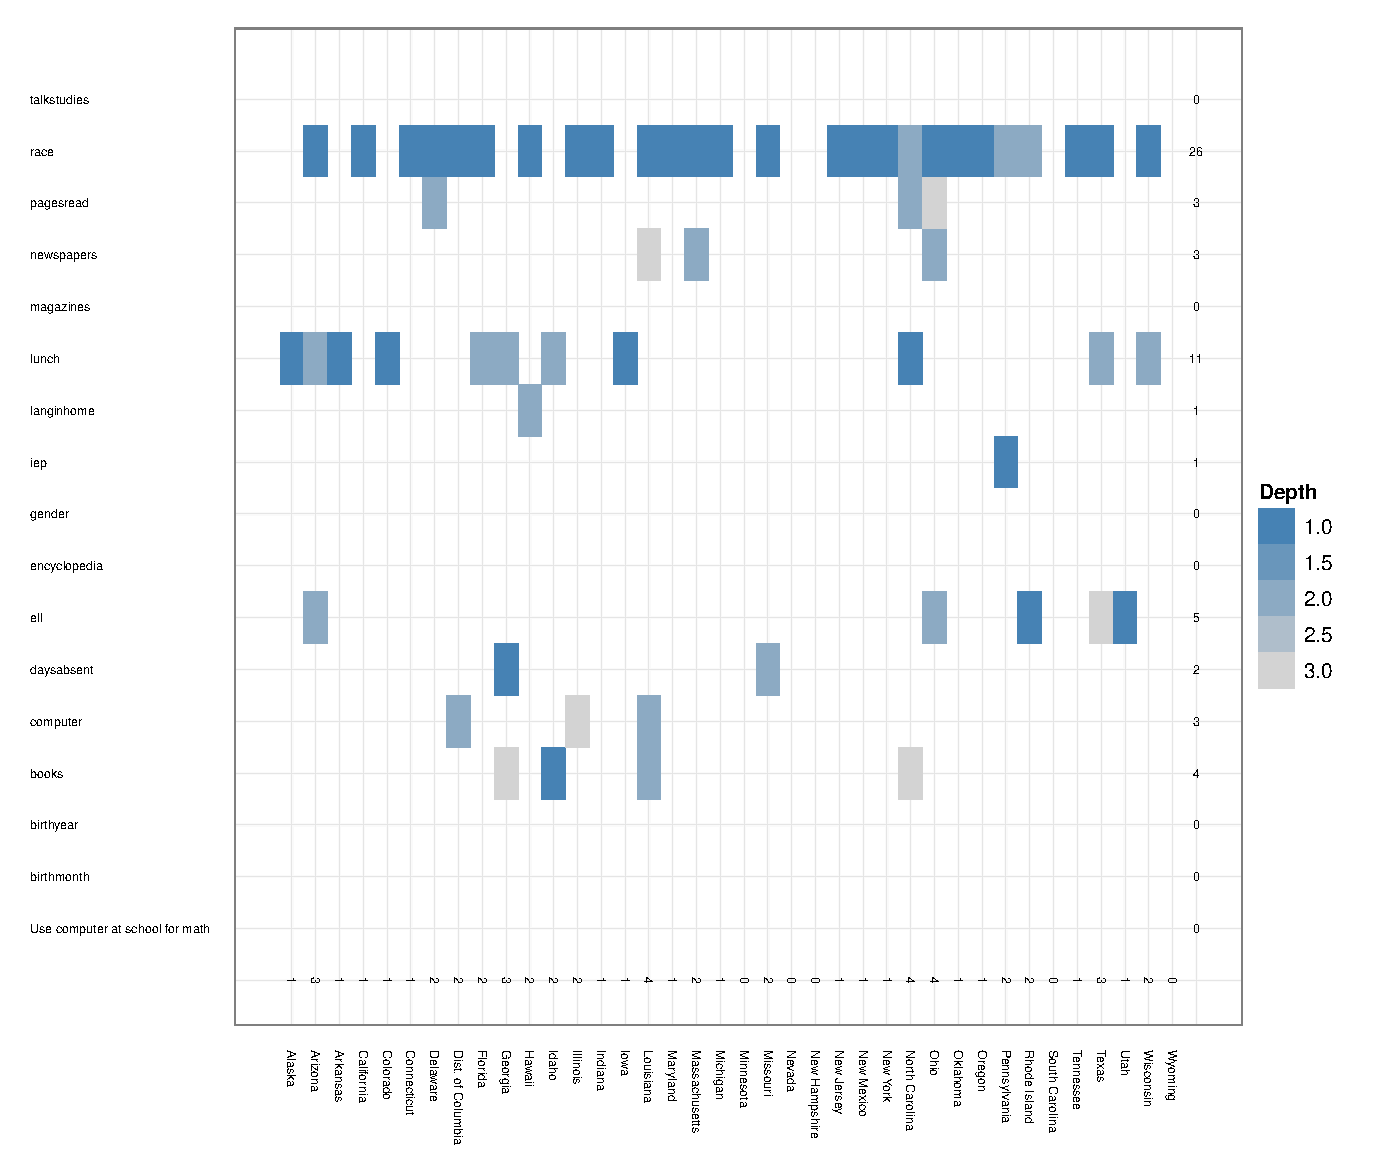
\includegraphics[width=\textwidth]{../Figures/g4mathtreeHeat.pdf}
\caption{Heat Map of Relative Importance of Covariates for Phase I: Grade 4 Math}
\label{fig:g4math:treeheat}
\end{center}
\end{figure}


%==================== Appendix J ====================================================================
\cleardoublepage
\addcontentsline{toc}{subsection}{Appendix J: Distribution of NAEP Scores for Matched vs. Unmatched Traditional Public School Students}
\subsection*{Appendix J\\Distribution of NAEP Scores for Matched vs. Unmatched Traditional Public School Students}
\label{appendixPublicDensity}

The figures in this appendix represent the distributions of matched and unmatched public school students as identified by the full logistic regression model. These models were chosen since they resulted in the largest number of unmatched traditional public school students vis-\`a-vis stratification. It should be noted that for some states there may be only one density line. This indicates that all traditional public school students within that state were either all matched or all not matched.

\begin{figure}[h]
\begin{center}
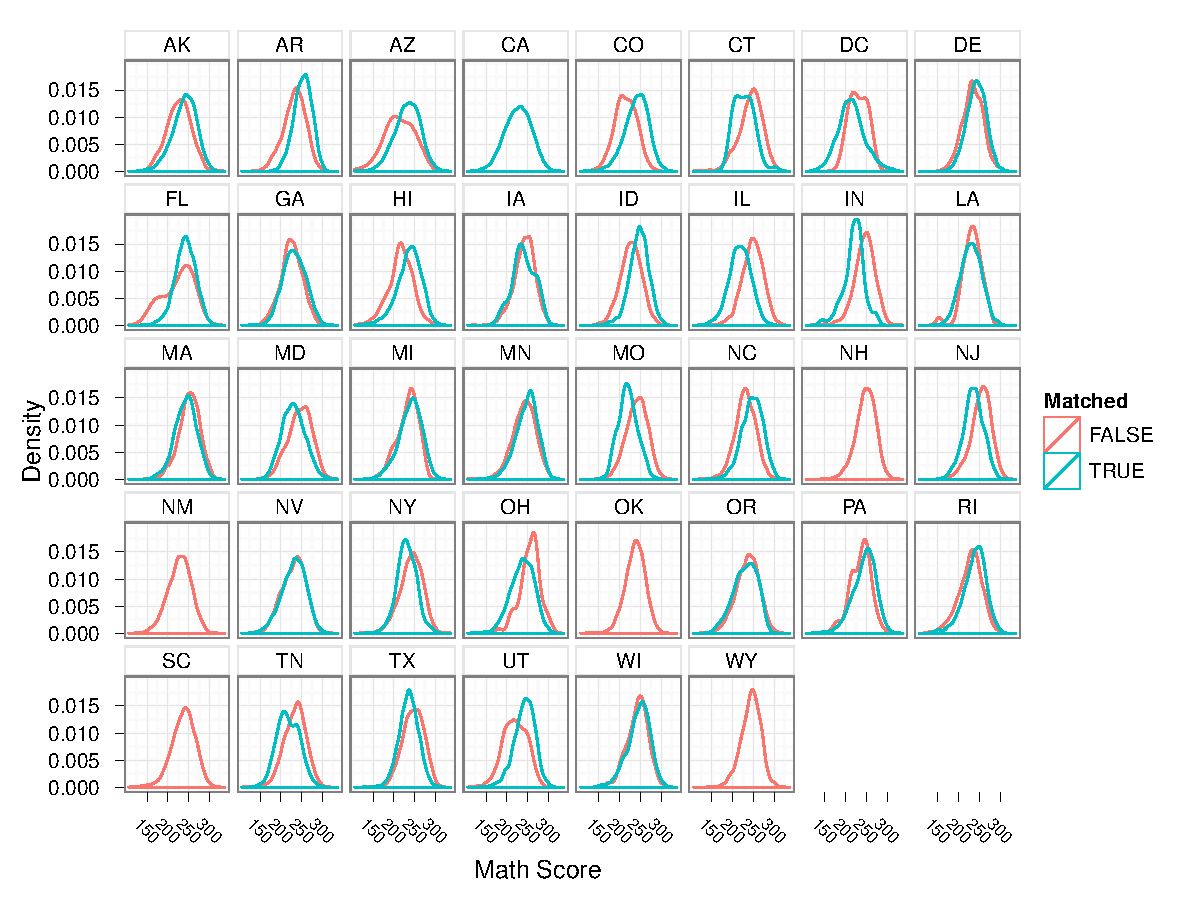
\includegraphics[width=\textwidth,angle=90]{../Figures/g4mathlrPublicDensity.pdf}
\caption{Density Distribution of Grade 4 Math: Matched vs. Unmatched Traditional Public School Students}
\label{fig:g4reading:publicdensity}
\end{center}
\end{figure}
\clearpage


%==================== Appendix K ====================================================================
\cleardoublepage
\addcontentsline{toc}{subsection}{Appendix K: Tables of Overall Results}
\subsection*{Appendix K\\Tables of Overall Results}
\label{appendixOverallResultsTables}

% latex table generated in R 2.12.2 by xtable 1.5-6 package
% Sun Jun 26 09:06:41 2011
\begin{table}[ht]
\begin{center}
\caption{Summary Propensity Score Analysis using Stratification}
\label{overallresults}
\begin{tabular}{lrrrrrrr}
  \hline
  & \multicolumn{ 2}{c}{Adjusted Mean} &  & \multicolumn{1x}{c}{} &  &  & \multicolumn{1}{c}{} \\ \cline{2-3} & Public & Charter & Diff & ATE & \textit{n} & \multicolumn{2}{c}{95\% CI} \\ \hline  & \multicolumn{7}{c}{Grade 4 Math} \\ \cline{2-8} \hline
Logistic Regression & 237.95 & 237.38 & -0.57 & -0.57 & 146656.00 & -1.72 & 0.57 \\ 
  Logistic Regression Step AIC & 237.96 & 237.35 & -0.60 & -0.60 & 146656.00 & -1.73 & 0.52 \\ 
  Conditional Inference Trees & 237.93 & 238.27 & 0.34 & 0.34 & 146638.00 & -0.96 & 1.64 \\ 
    & \multicolumn{7}{c}{Grade 4 Reading} \\ \cline{2-8}Logistic Regression & 218.27 & 218.96 & 0.70 & 0.70 & 141352.00 & -0.71 & 2.11 \\ 
  Logistic Regression Step AIC & 218.26 & 219.22 & 0.96 & 0.96 & 141352.00 & -0.44 & 2.37 \\ 
  Conditional Inference Trees & 218.26 & 219.01 & 0.75 & 0.75 & 141340.00 & -0.62 & 2.12 \\ 
    & \multicolumn{7}{c}{Grade 8 Math} \\ \cline{2-8}Logistic Regression & 278.77 & 279.10 & 0.33 & 0.33 & 97563.00 & -1.40 & 2.06 \\ 
  Logistic Regression Step AIC & 278.77 & 279.54 & 0.77 & 0.77 & 97563.00 & -0.91 & 2.46 \\ 
  Conditional Inference Trees & 278.72 & 280.89 & 2.17 & 2.17 & 97521.00 & 0.36 & 3.98 \\ 
    & \multicolumn{7}{c}{Grade 8 Reading} \\ \cline{2-8}Logistic Regression & 259.80 & 262.82 & 3.02 & 3.02 & 105486.00 & 1.55 & 4.49 \\ 
  Logistic Regression Step AIC & 259.80 & 262.67 & 2.87 & 2.87 & 105486.00 & 1.36 & 4.38 \\ 
  Conditional Inference Trees & 259.75 & 265.39 & 5.65 & 5.65 & 105468.00 & 4.36 & 6.93 \\ 
   \hline
\end{tabular}
\end{center}
\end{table}

% latex table generated in R 2.12.2 by xtable 1.5-6 package
% Sun Jun 26 10:05:22 2011
\begin{table}[ht]
\begin{center}
\caption{Summary of Propensity Score Matching}
\begin{tabular}{rrrr@{}lrrr}
  \hline
  M & Charter & Public & \multicolumn{2}{c}{Diff} & ES & \multicolumn{2}{c}{95\% CI} \\ \hline  & \multicolumn{7}{c}{Grade 4 Math} \\ \cline{2-8}  1 & 233.10 & 231.92 & 1.17 &  & 0.04 & -0.01 & 2.36 \\ 
    5 & 233.94 & 232.88 & 1.06 & *** & 0.04 & 0.53 & 1.60 \\ 
   10 & 235.58 & 234.40 & 1.18 & *** & 0.04 & 0.79 & 1.57 \\ 
    & \multicolumn{7}{c}{Grade 4 Reading} \\ \cline{2-8}  1 & 213.33 & 212.09 & 1.24 &  & 0.04 & -0.26 & 2.74 \\ 
    5 & 214.35 & 213.06 & 1.29 & *** & 0.04 & 0.60 & 1.99 \\ 
   10 & 215.89 & 214.45 & 1.44 & *** & 0.04 & 0.93 & 1.95 \\ 
    & \multicolumn{7}{c}{Grade 8 Math} \\ \cline{2-8}  1 & 273.64 & 269.94 & 3.70 & *** & 0.10 & 2.11 & 5.29 \\ 
    5 & 276.14 & 272.56 & 3.58 & *** & 0.10 & 2.83 & 4.34 \\ 
   10 & 277.42 & 274.11 & 3.31 & *** & 0.09 & 2.75 & 3.87 \\ 
    & \multicolumn{7}{c}{Grade 8 Reading} \\ \cline{2-8}  1 & 259.93 & 254.63 & 5.30 & *** & 0.16 & 3.92 & 6.68 \\ 
    5 & 261.50 & 255.63 & 5.87 & *** & 0.17 & 5.21 & 6.52 \\ 
   10 & 262.22 & 256.76 & 5.46 & *** & 0.16 & 4.97 & 5.94 \\ 
   \hline \multicolumn{8}{l}{*\textit{p} $<$ .05; **\textit{p} $<$ .01; ***\textit{p} $<$ .001} \\ \end{tabular}
\end{center}
\end{table}

\begin{table}[ht]
\caption{Summary of Multilevel PSA}
\begin{center}
\begin{tabular}{lrrrrrrrr}
\hline
 & \multicolumn{ 2}{c}{Adjusted Mean} &  & \multicolumn{1}{c}{} &  &  & \multicolumn{1}{c}{} \\ \cline{2-3}
 & Public & Charter & Diff & ATE & \textit{n} & \multicolumn{2}{c}{95\% CI} \\ \hline
 & \multicolumn{ 7}{c}{Grade 4 Math} \\ \cline{2-8}
Logistic Regression & 236.51 & 236.55 & 3.40 & 0.04 & 83241 & -1.50 & 1.58 \\ 
Logistic Regression Step AIC & 237.25 & 236.83 & 4.22 & -0.41 & 95290 & -2.05 & 1.23 \\ 
Conditional Inference Trees & 236.70 & 237.78 & 3.89 & 1.10 & 118812 & -0.26 & 2.54 \\
% Matching &  &  &  &  &  &  &  &  \\ 
 & \multicolumn{ 7}{c}{Grade 4 Reading} \\ \cline{2-8}
Logistic Regression & 217.14 & 216.87 & 4.65 & -0.27 & 80465 & -2.29 & 1.75 \\ 
Logistic Regression Step AIC & 217.05 & 217.46 & 4.71 & 0.41 & 86885 & -1.52 & 2.33 \\ 
Conditional Inference Trees & 216.09 & 220.92 & 5.99 & 4.83 & 108938 & 2.91 & 6.75 \\
% Matching &  &  &  &  &  &  &  &  \\
 & \multicolumn{ 7}{c}{Grade 8 Math} \\ \cline{2-8}
Logistic Regression & 278.13 & 277.90 & 5.31 & -0.23 & 61795 & -2.41 & 1.94 \\
Logistic Regression Step AIC & 278.62 & 280.52 & 6.07 & 1.90 & 69535 & -0.33 & 4.13 \\
Conditional Inference Trees & 277.61 & 281.11 & 5.28 & 3.50 & 80594 & 1.48 & 5.52 \\
%Matching &  &  &  &  &  &  &  & \multicolumn{1}{l}{} \\
 & \multicolumn{ 7}{c}{Grade 8 Reading} \\ \cline{2-8}
Logistic Regression & 258.97 & 263.19 & 4.14 & 4.22 & 71270 & 2.45 & 5.99 \\
Logistic Regression Step AIC & 259.25 & 263.61 & 4.25 & 4.36 & 77513 & 2.58 & 6.14 \\
Conditional Inference Trees & 258.10 & 264.97 & 4.37 & 6.87 & 84352 & 5.12 & 8.63 \\
%Matching &  &  &  &  &  &  &  & \multicolumn{1}{l}{} \\ 
\hline
\end{tabular}
\label{overallresults}
\end{center}
\end{table}



\end{document}
